\chapter{Experimentaciones y Resultados}\label{chapter:results}

En la presente sección comenzaremos mostrando los sistemas de cómputo utilizados para la experimentación.
Seguidamente, dividimos este capítulo en seis secciones.
Primero, se muestra los resultados de la optimización del \emph{bend}.
Para ello se inicia mostrando en tres gráficas distintas el desempeño de cada algoritmo en 
las tres etapas de la estrategia de optimización; luego se detalla los resultados por cada algoritmo
de manera individual.
Segundo, se realiza un análisis al diseño del \emph{bend} mejor optimizado.
Tercero, de manera similar al caso del \emph{bend}, se expone los resultado de la optimización del WDM.
Cuarto, se desarrolla un análisis al diseño del WDM mejor optimizado.
Quinto, se realiza una discusión crítica sobre los resultados de la optimización del \emph{bend}.
Finalmente, se realiza una discusión similar sobre los resultados del WDM.

Los experimentos se realizaron en tres equipos brindados por la Universidad de Ingeniería y Tecnología:

\begin{enumerate}
  \item Un Intel Core i7-3770K 3.50 GHz con 8 cores y 32 GB de RAM.
        Este computador contó con un GPU NVIDIA Quadro RTX 4000 con 8GB GDDR6.

  \item Del \emph{cluster} Khipu, un Intel Xeon Gold 6230 2.10 GHz con 40 \emph{cores} y 128 GB de RAM.
        Este nodo contó con un GPU NVIDIA Tesla T4 con 16 GB GDDR6.

  \item Del \emph{cluster} Khipu, un AMD EPYC 7742 2.25 GHz con 128 \emph{cores} y 1024 GB de RAM.
        Este nodo contó con un GPU NVIDIA Ampere A100 con 40 GB HMB2.

\end{enumerate}

Sacando la media geométrica de los tiempos calculados, el tiempo promedio de ejecución en los tres 
sistemas en cada etapa de la estrategia de optimización se detalla en la \autoref{tab:times} (el signo -
indica que en ese sistema de cómputo no se realizaron experimentos con ese dispositivo).

\begin{table}[ht]
    \centering
    \begin{tabular}{|c|c|c|c|}
    \hline 
      Tiempo promedio &  Quadro RTX (s) & Tesla T4 & Ampere A100 \\
    \hline 
      Optimización continua (\emph{bend})            & 14.261 & 15.432 & - \\
      Optimización discreta (\emph{bend})            & 15.961 & 18.718 & - \\
      Optimización de fabricación (\emph{bend})      & 47.084 & 50.639 & - \\
      Optimización continua (WDM)                    & 16.876 & - & 17.479 \\
      Optimización discreta (WDM)                    & 18.431 & - & 19.780 \\
      Optimización de fabricación (WDM)              & 53.941 & - & 55.406 \\
    \hline 
    \end{tabular}
    \caption{Tiempos promedios de ejecución en cada etapa de optimización para el \emph{bend} y WDM con los
    tres sistemas de cómputo usados.}
    \label{tab:times}
\end{table}

Por cada optimización se realizó como máximo $2000$ evaluaciones de $f_{obj}$ en la optimización continua,
$3 \times 800$ en la optimización discreta y $3 \times 400$ en la optimización de fabricación.
Así, por ejemplo, usando Quadro RTX la optimización de un \emph{bend} podía tomar hasta 34 horas
y usando Ampere A100 la optimización de un WDM podía tomar hasta 41 horas.

Por otro lado, cada GPU solo puede realizar una simulación a la vez, en caso de querer 
evaluar dos parametrizaciones al mismo tiempo una era puesta en cola. De este modo,
siendo el tiempo de simulación el cuello de botella de las optimizaciones, los programas simplemente
se ejecutaron con un solo \emph{core} y se limitó la memoria a 32 GB para los nodos del \emph{cluster}
Khipu mediante SLURM (herramienta que funciona como gestor de recursos de Khipu).


En las siguientes secciones las imágenes que muestran resultados del \emph{bend} o WDM
incluyen un círculo blanco, este representa una circunferencia de radio $r_f = 80 nm$,
el mínimo radio de curvatura que se está intentando imponer.


\section{Resultados de Optimización del \emph{Bend}}\label{sec:results-bend}

En la \autoref{fig:bend-cont}, \autoref{fig:bend-disc} y \autoref{fig:bend-fab} se observa 
el desempeño de los cinco algoritmos seleccionados en la etapa de optimización continua, discreta y
de fabricación del \emph{bend}, respectivamente.
Los resultados en más detalle por algoritmo se pueden encontrar en la 
\autoref{tab:opt-LBFGSB-bend} (L-BFGS-B),
\autoref{tab:opt-CMA-bend} (G-CMA-ES),
\autoref{tab:opt-MMA-bend} (MMA),
\autoref{tab:opt-PSO-bend} (G-PSO) y
\autoref{tab:opt-GA-bend} (G-GA).

\begin{landscape}
\begin{figure}[ht]
  \centering
  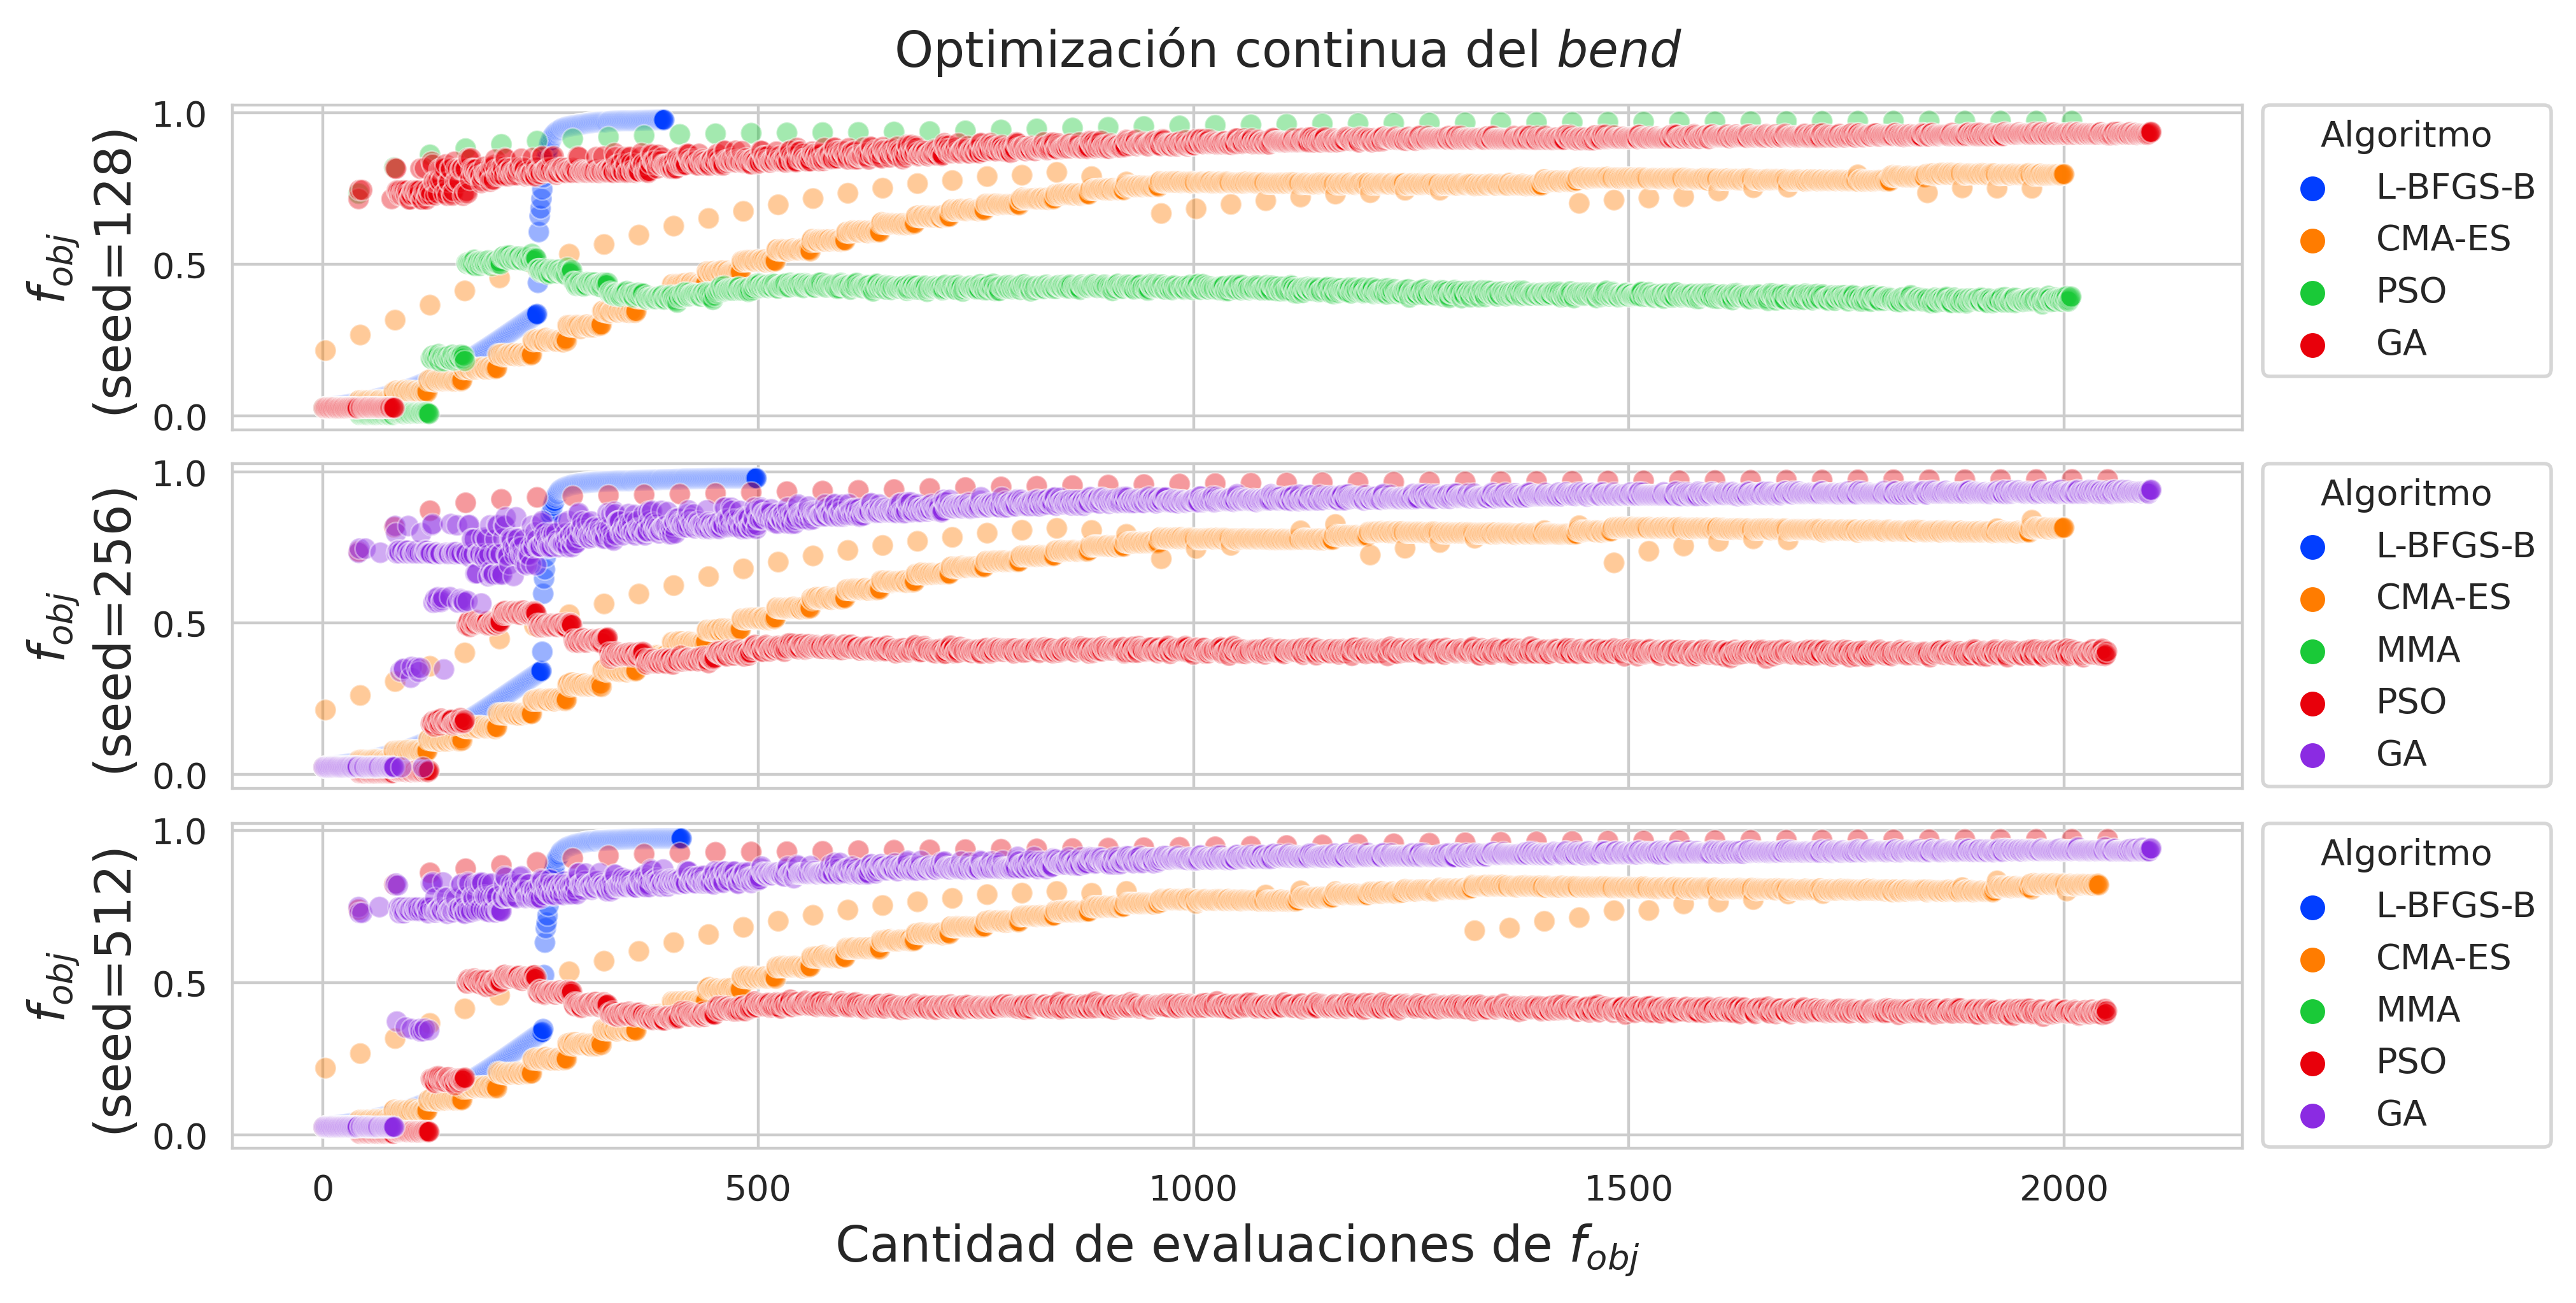
\includegraphics[scale=1.0]{image/results/bend/bend-opt-cont.png}
  \caption{Gráfico de valores de $f_{obj}$ obtenidos por los algoritmos en la optimización continua del \emph{bend}}
  \label{fig:bend-cont}
\end{figure}
\end{landscape}

\begin{landscape}
\begin{figure}[ht]
  \centering
  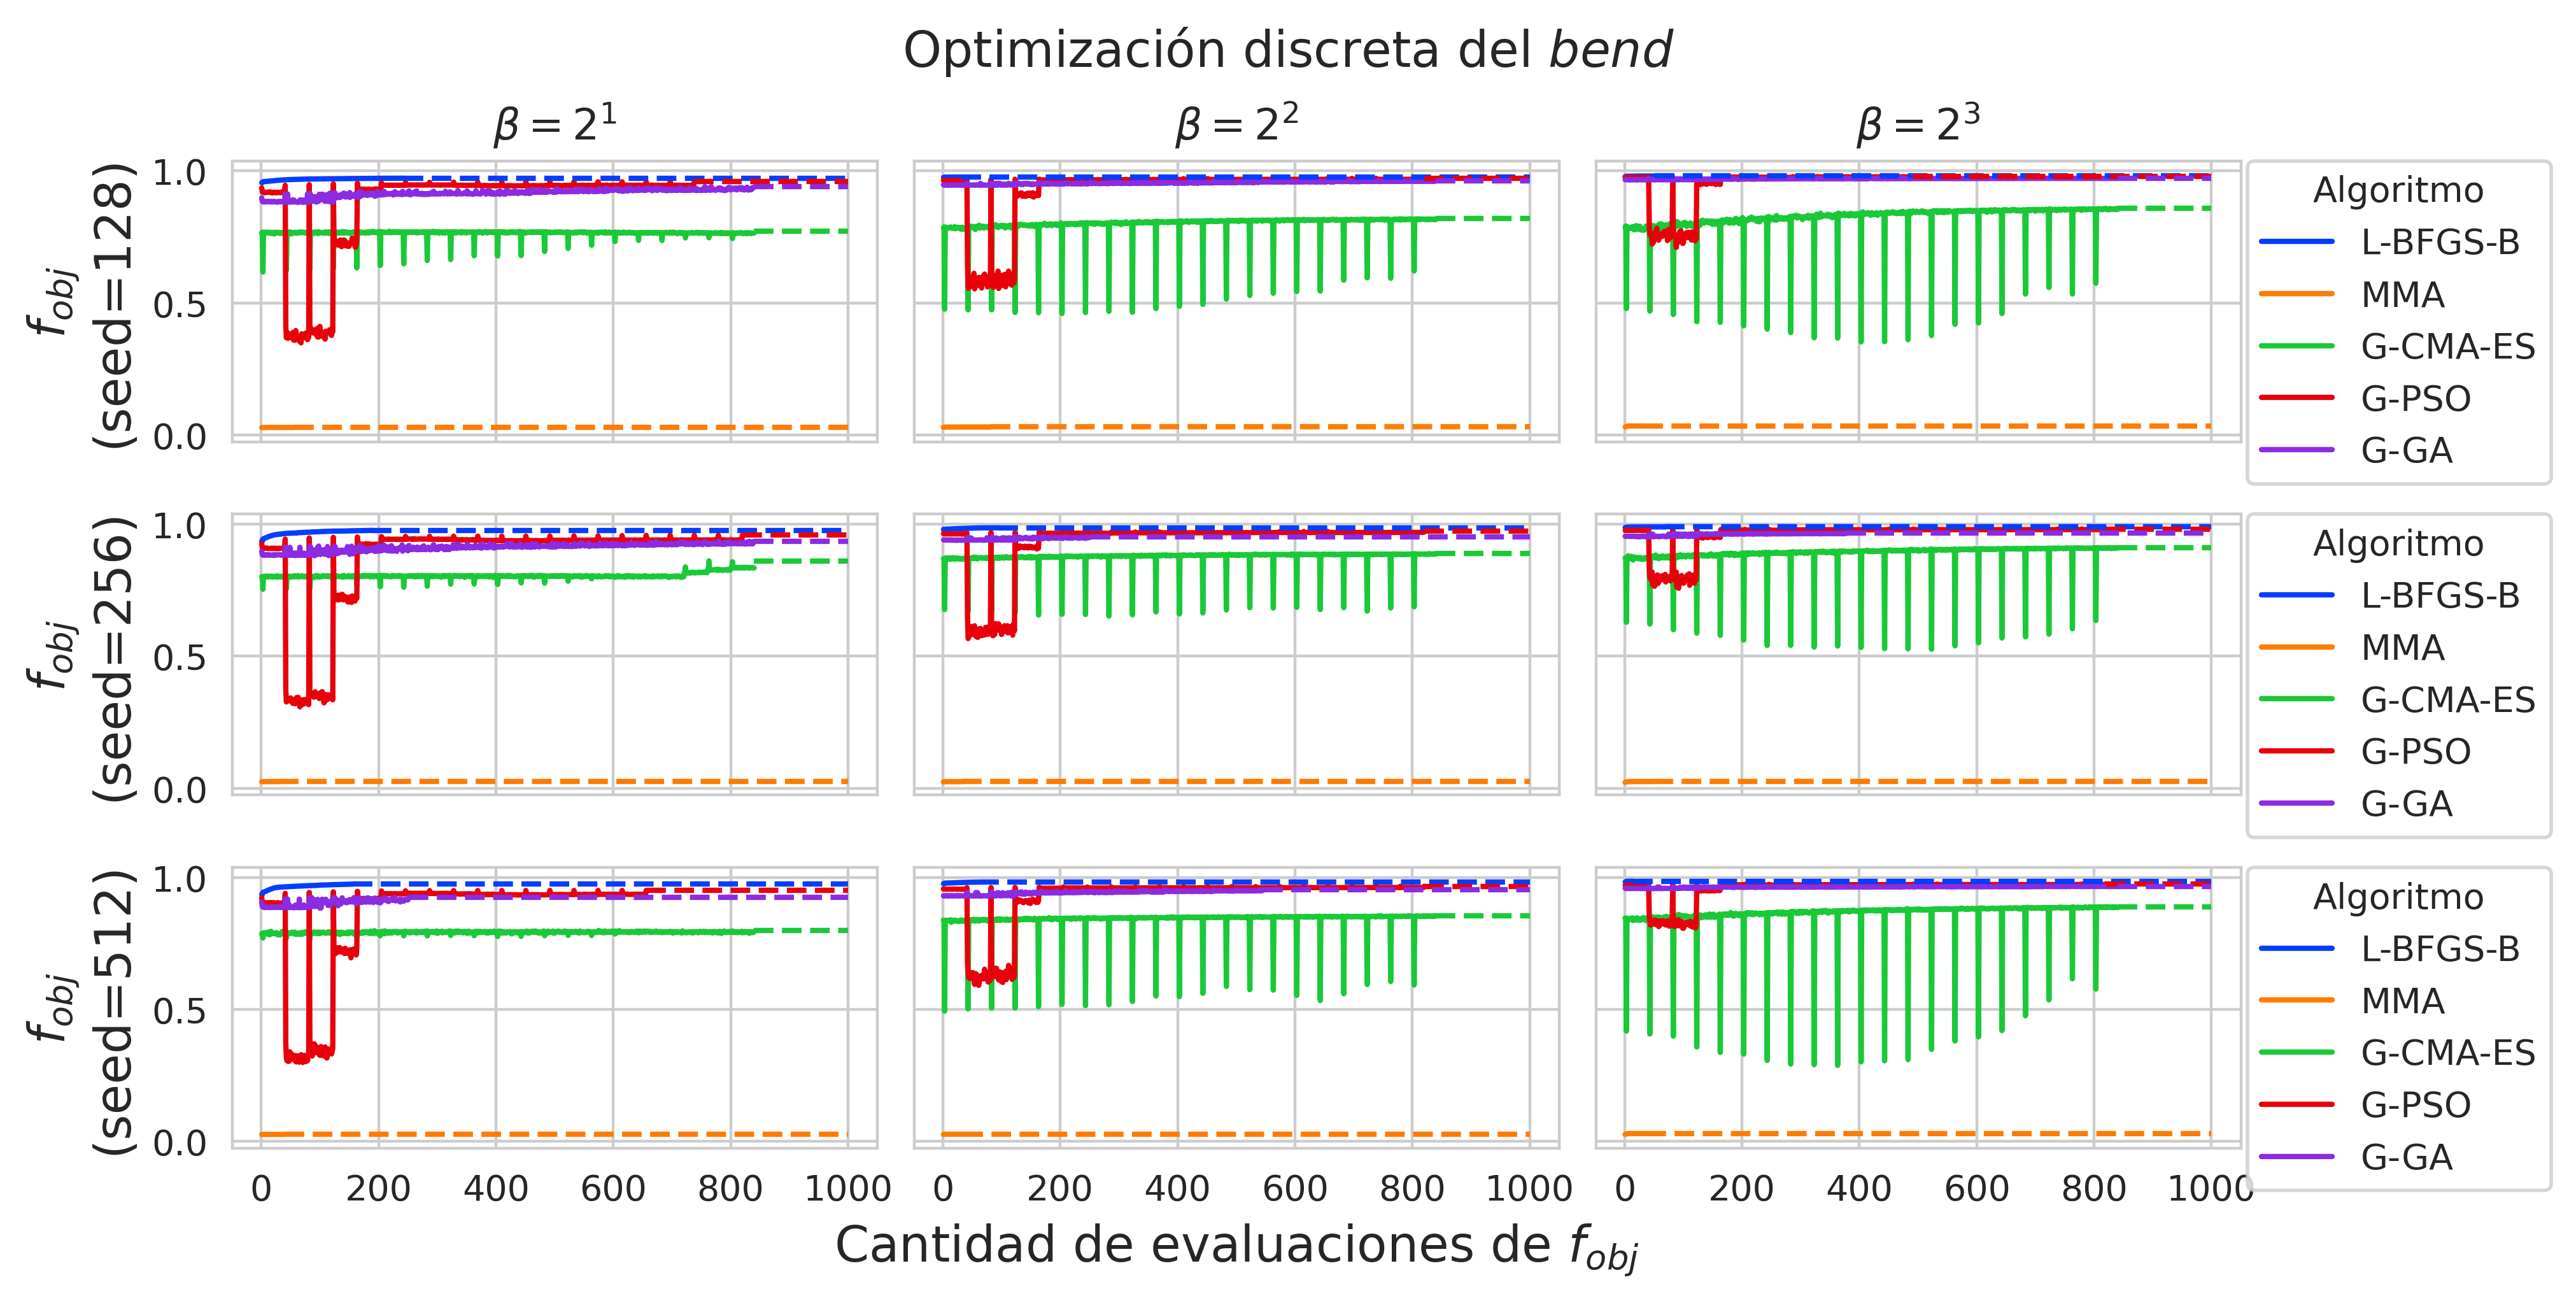
\includegraphics[scale=1.0]{image/results/bend/bend-opt-disc.png}
  \caption{Gráfico de valores de $f_{obj}$ obtenidos por los algoritmos en la optimización discreta del \emph{bend}}
  \label{fig:bend-disc}
\end{figure}
\end{landscape}

\begin{landscape}
\begin{figure}[ht]
  \centering
  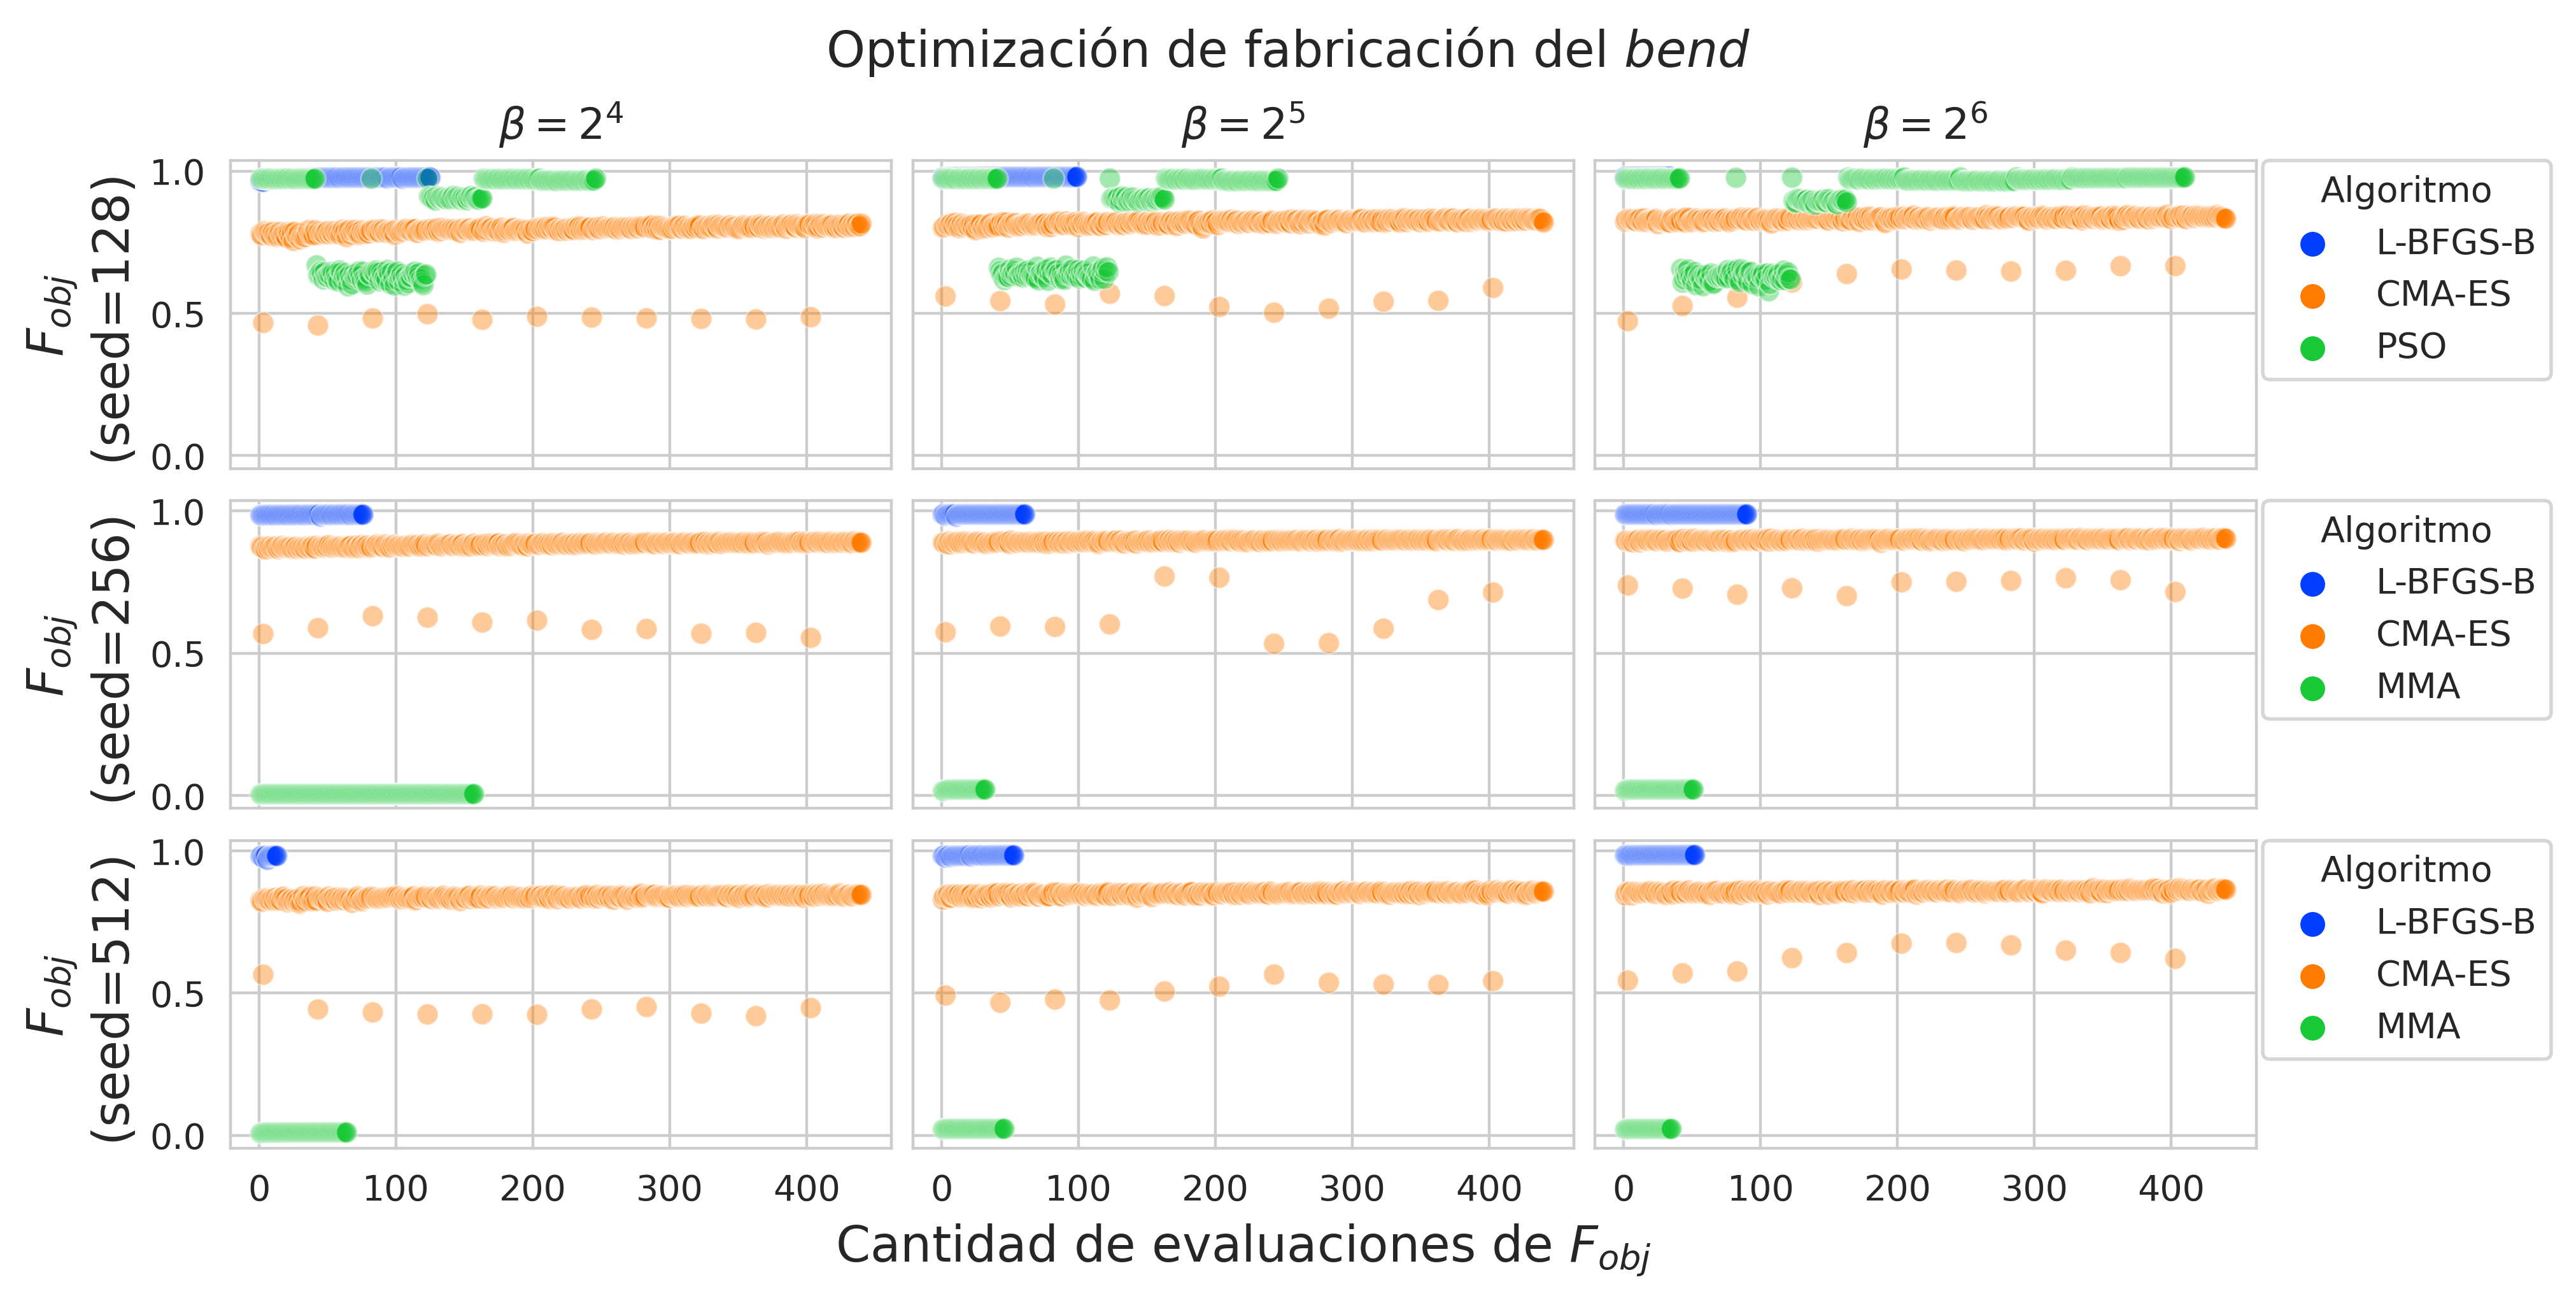
\includegraphics[scale=1.0]{image/results/bend/bend-opt-fab.png}
  \caption{Gráfico de valores de $F_{obj}$ obtenidos por los algoritmos en la optimización de fabricación del \emph{bend}}
  \label{fig:bend-fab}
\end{figure}
\end{landscape}

\section{Diseño del \emph{Bend} Mejor Optimizado}\label{sec:best-bend}

De la sección anterior tenemos que el \emph{bend} mejor optimizado se consiguió
utilizando el algoritmo L-BFGS-B con un \emph{seed} (valor de semilla) de 256.

Al aplicar la \autoref{eq:grayscale} obtenemos que el porcentage de región gris en el diseño
es de 1.097 \%, un valor menor a 2 \%, por lo cual podemos considerar que el diseño ha sido
correctamente binarizado. Por otro lado, si eliminamos las regiones no conectadas con la guía de entrada
tenemos un diseño con un porcentaje de gris de 0.168 \%.
Estos diseños lo podemos observar en la \autoref{fig:bestbend}.
Adicionalmente, en la \autoref{fig:broadband-bend} se muestra el comportamiento del diseño
en un rango de longitudes de onda de $1500nm$ a $1600 nm$.

\begin{figure}[ht]
  \centering

  % 1° row
  \subfigure[Diseño nominal.]
  {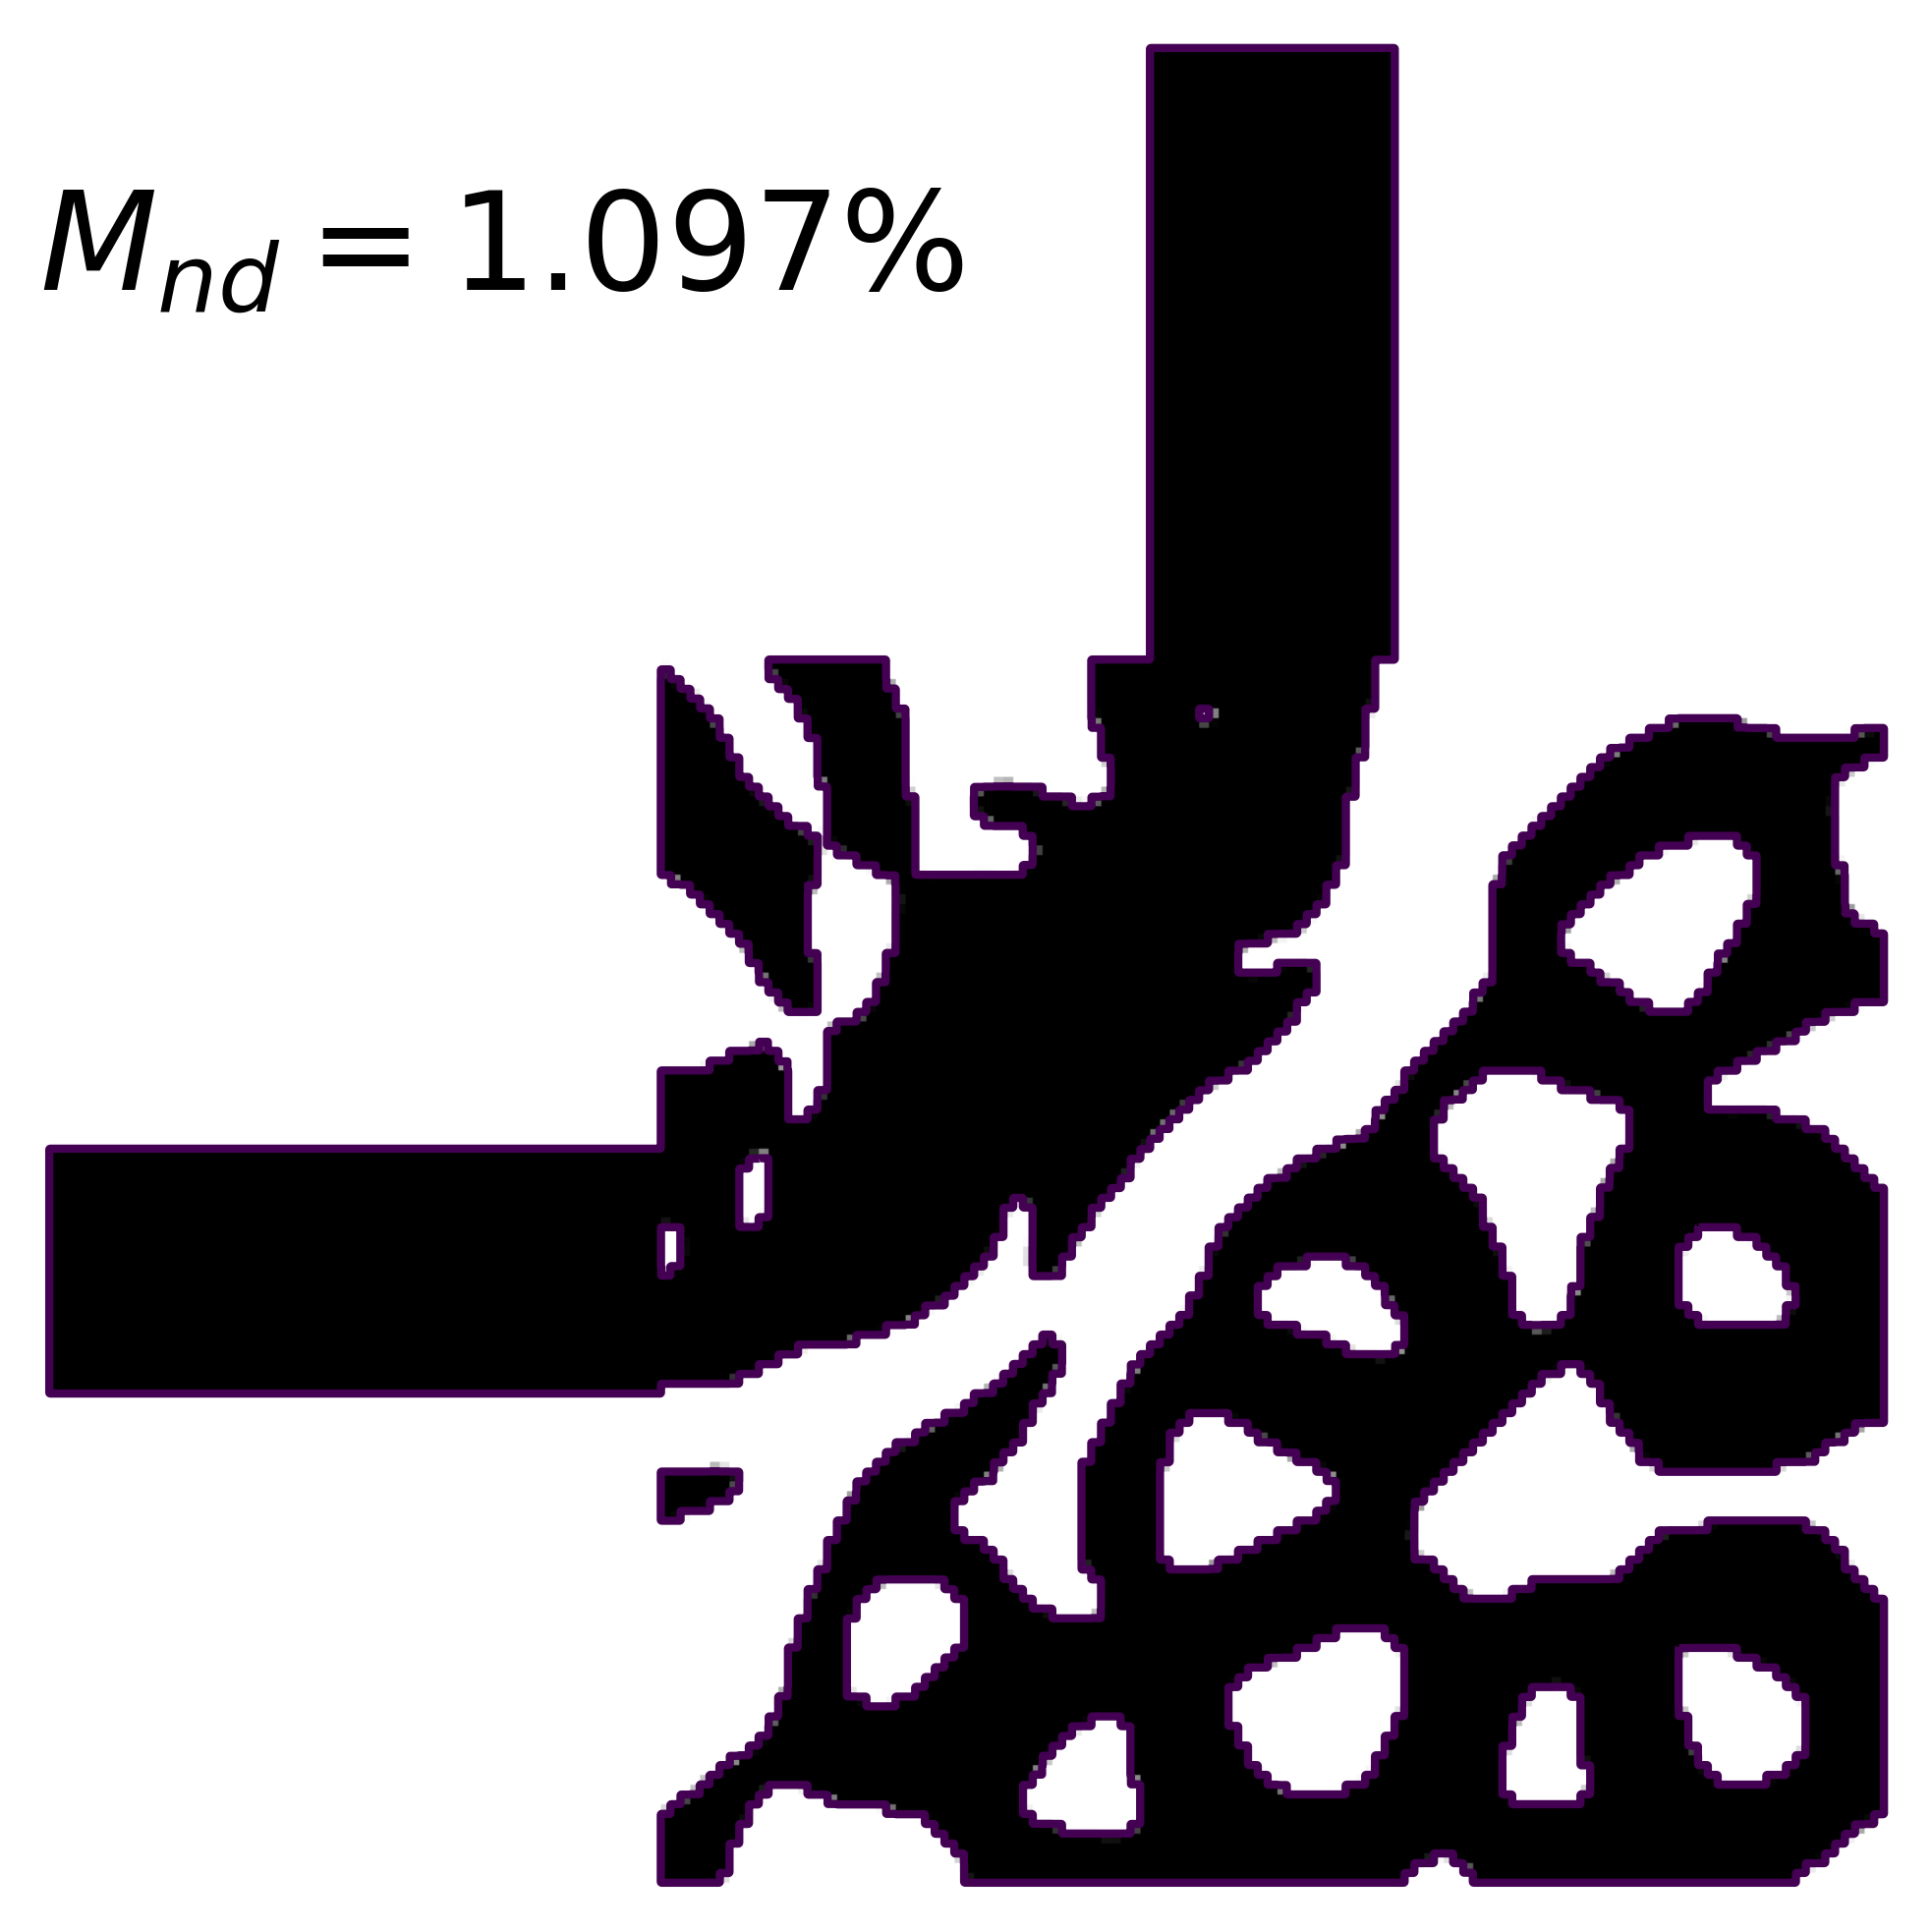
\includegraphics[width=0.35\textwidth]{image/results/bend/best/eps.png}}
  %\hfill
  \subfigure[Diseño nominal tras eliminar regiones no conexas.]{
    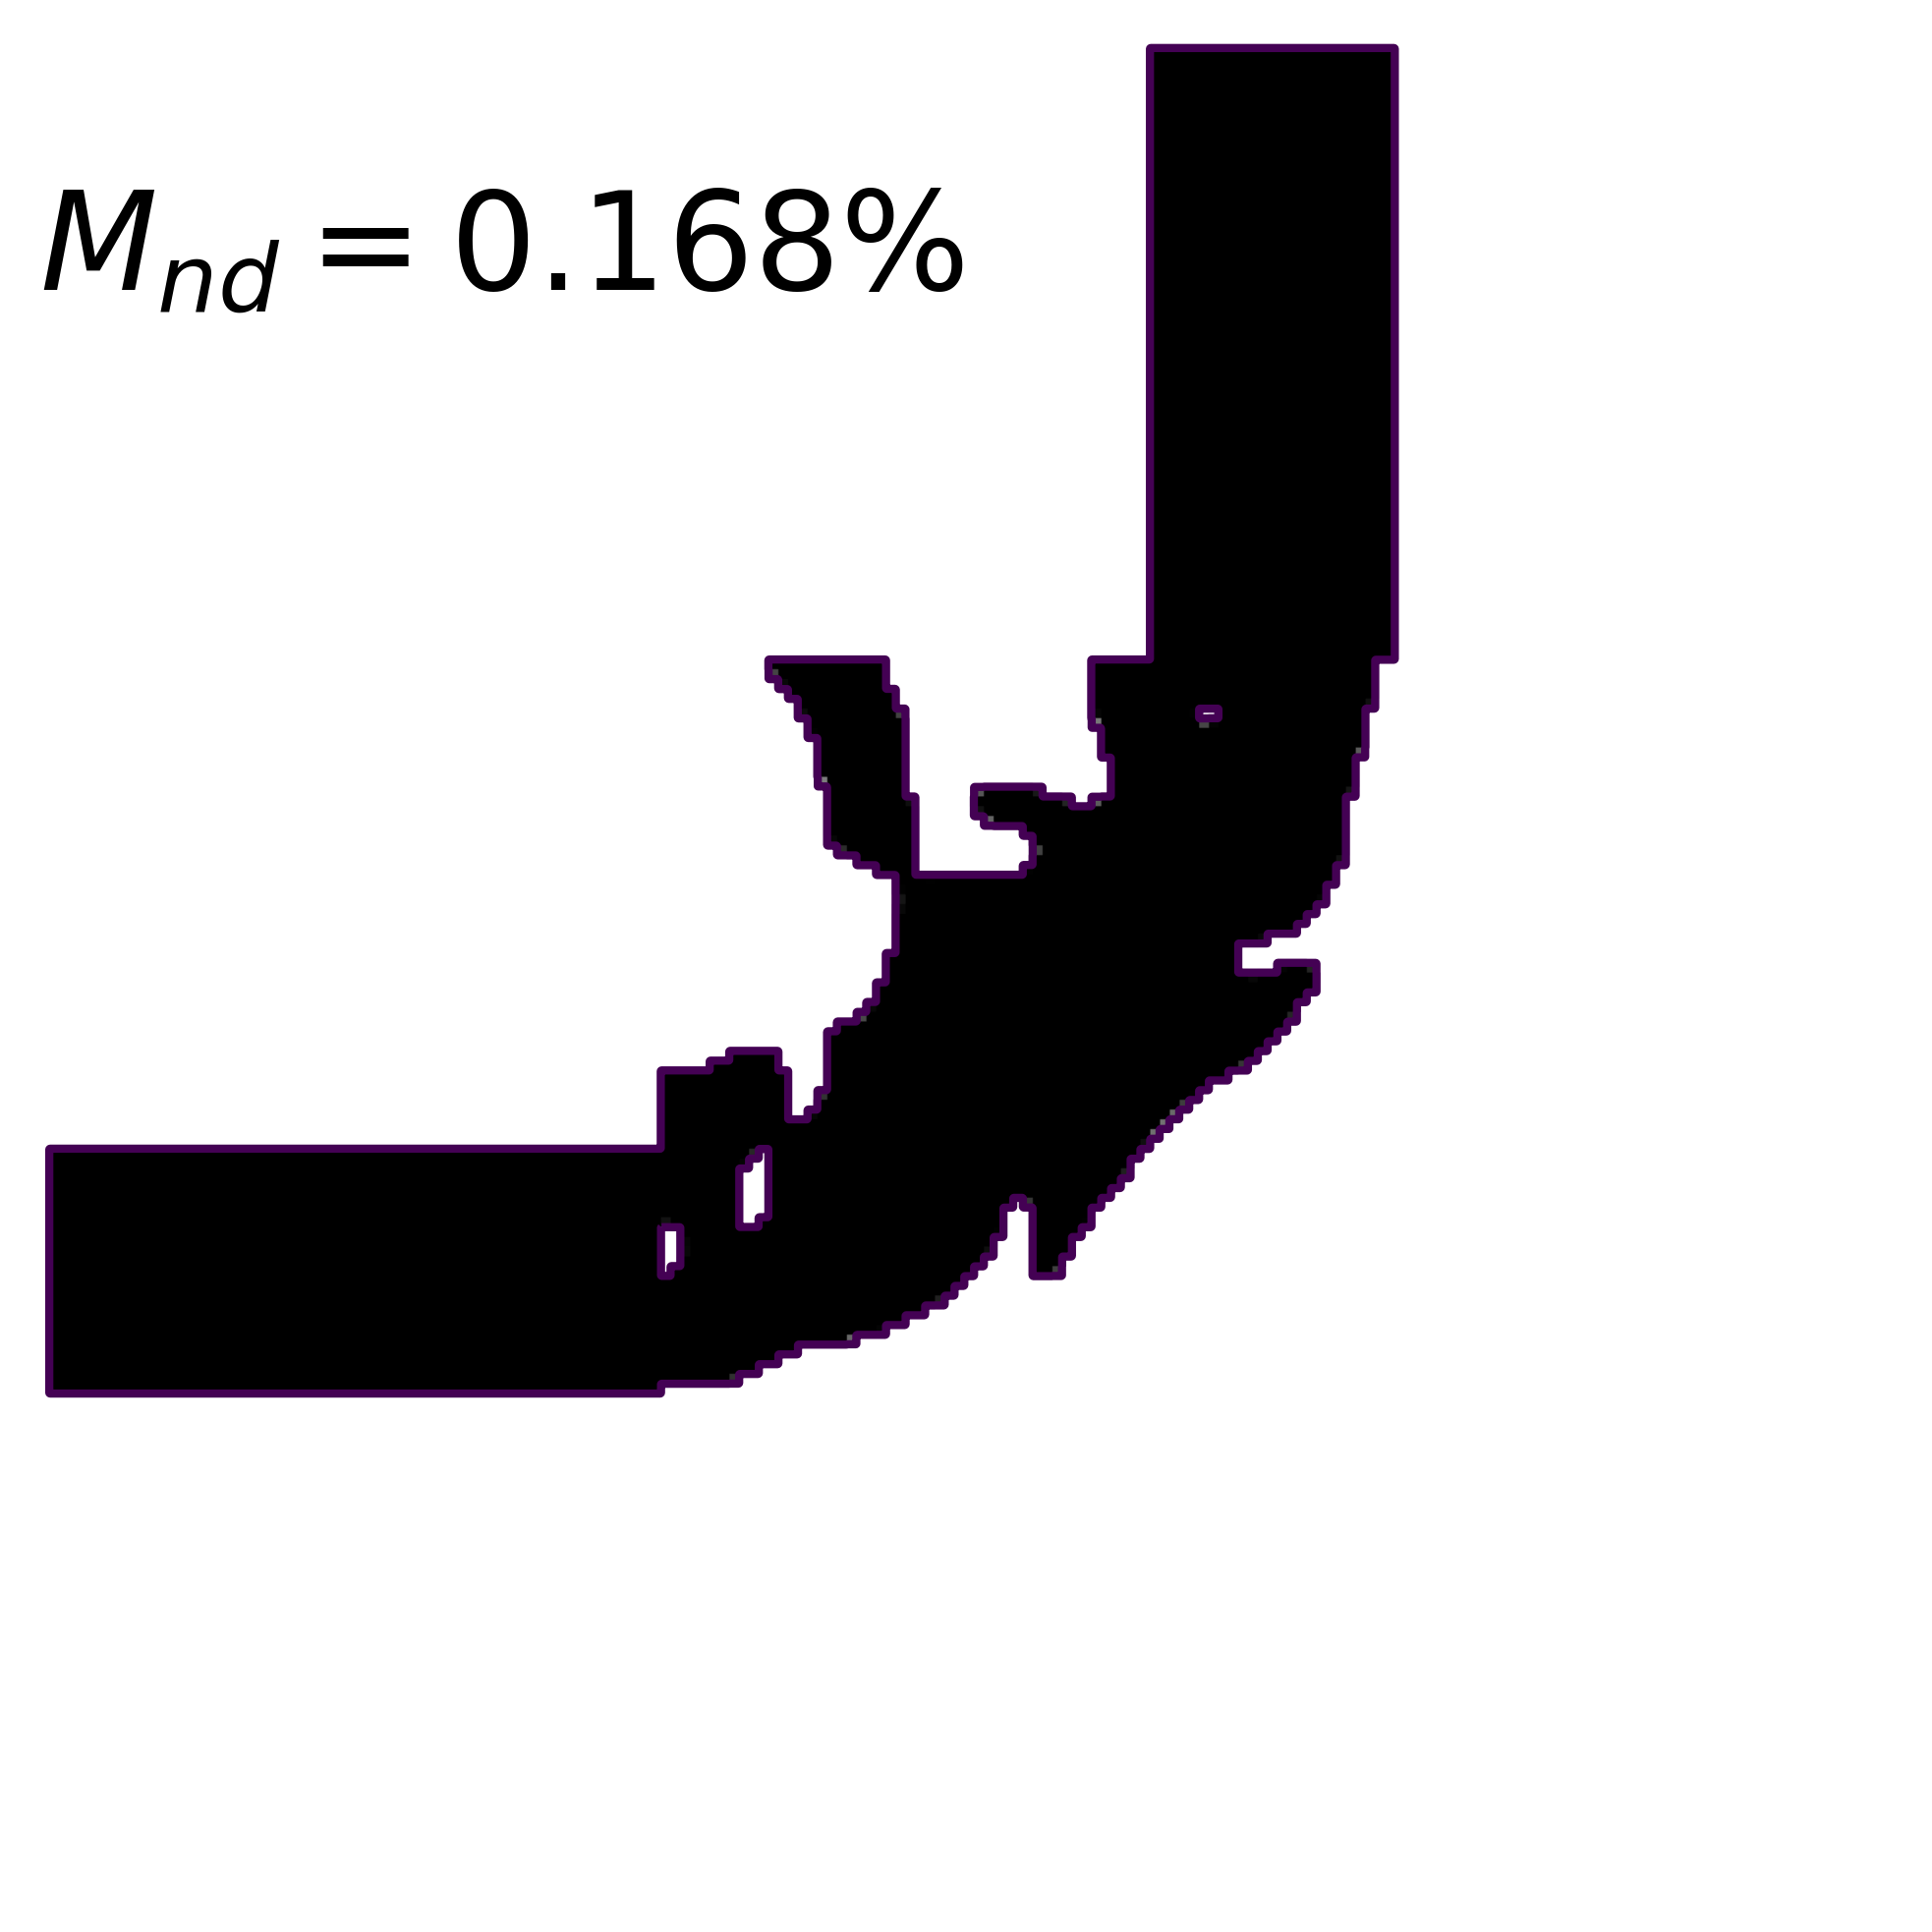
\includegraphics[width=0.35\textwidth]{image/results/bend/best/eps_post.png}
  }

  % 2° row
  \subfigure[Campo $|\boldsymbol{E}|^2$ del diseño nominal.]
  {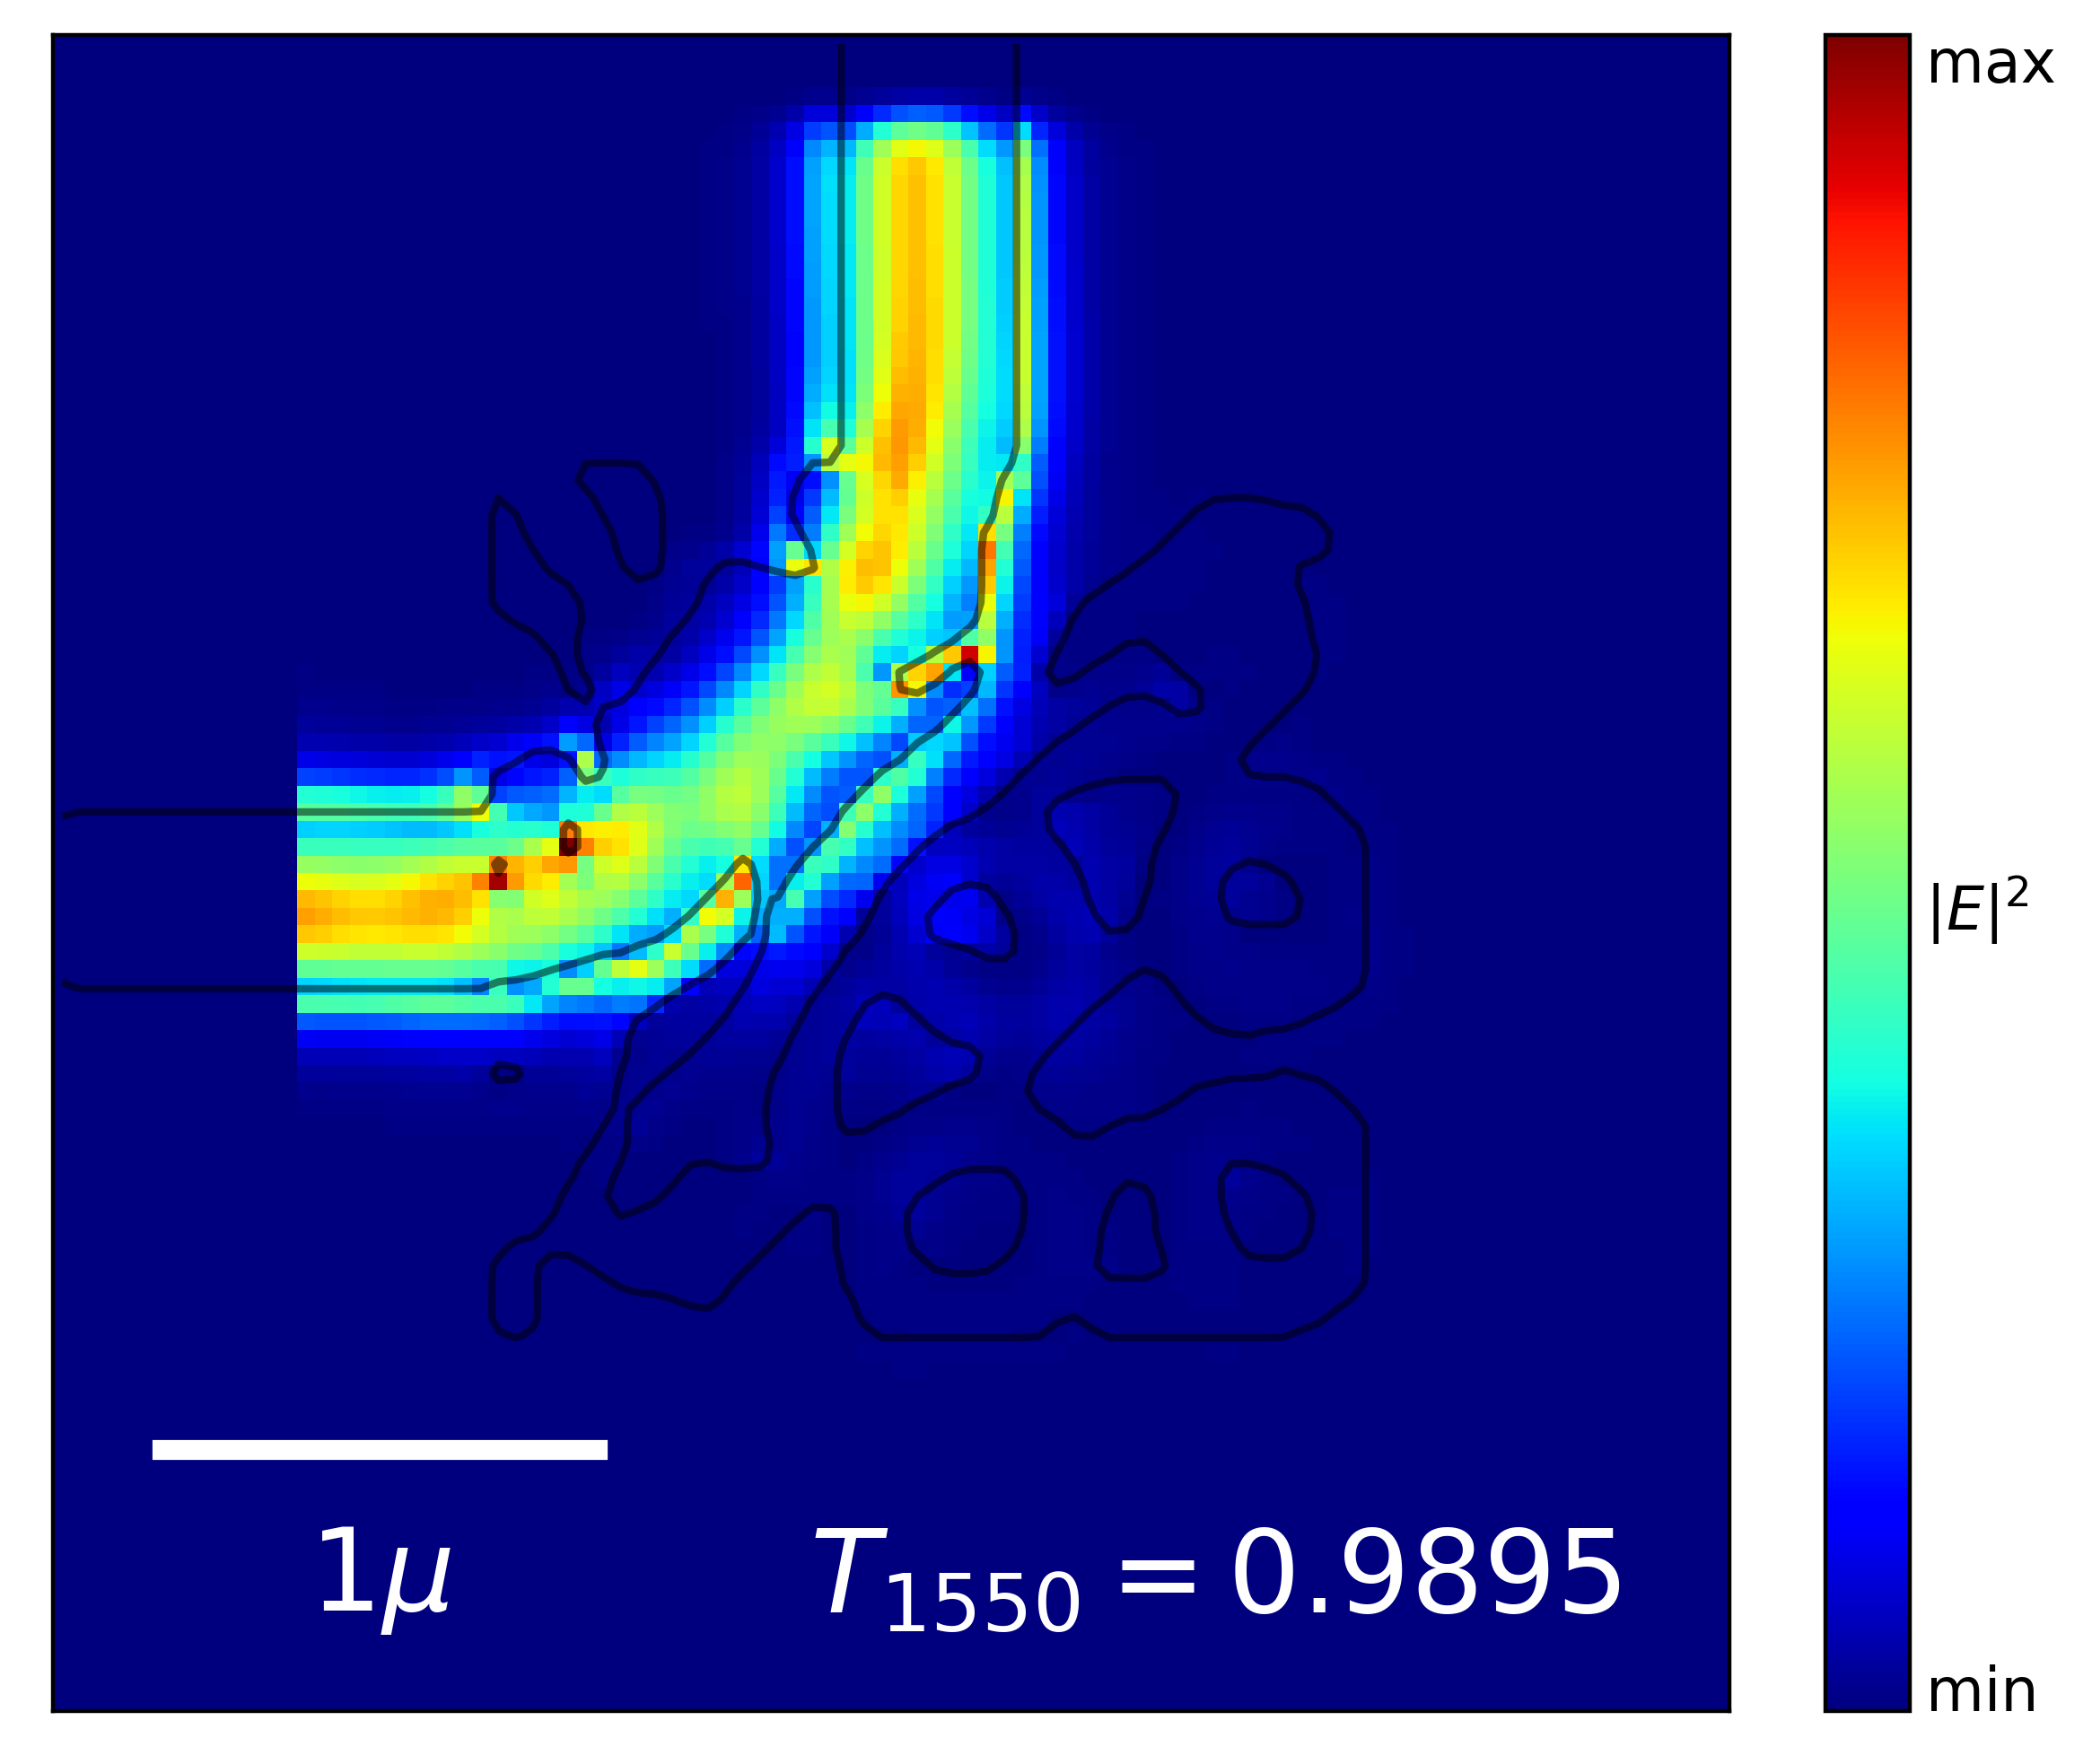
\includegraphics[width=0.35\textwidth]{image/results/bend/best/field.png}}
  %\hfill
  \subfigure[Campo $|\boldsymbol{E}|^2$ del diseño nominal tras eliminar regiones no conexas.]{
    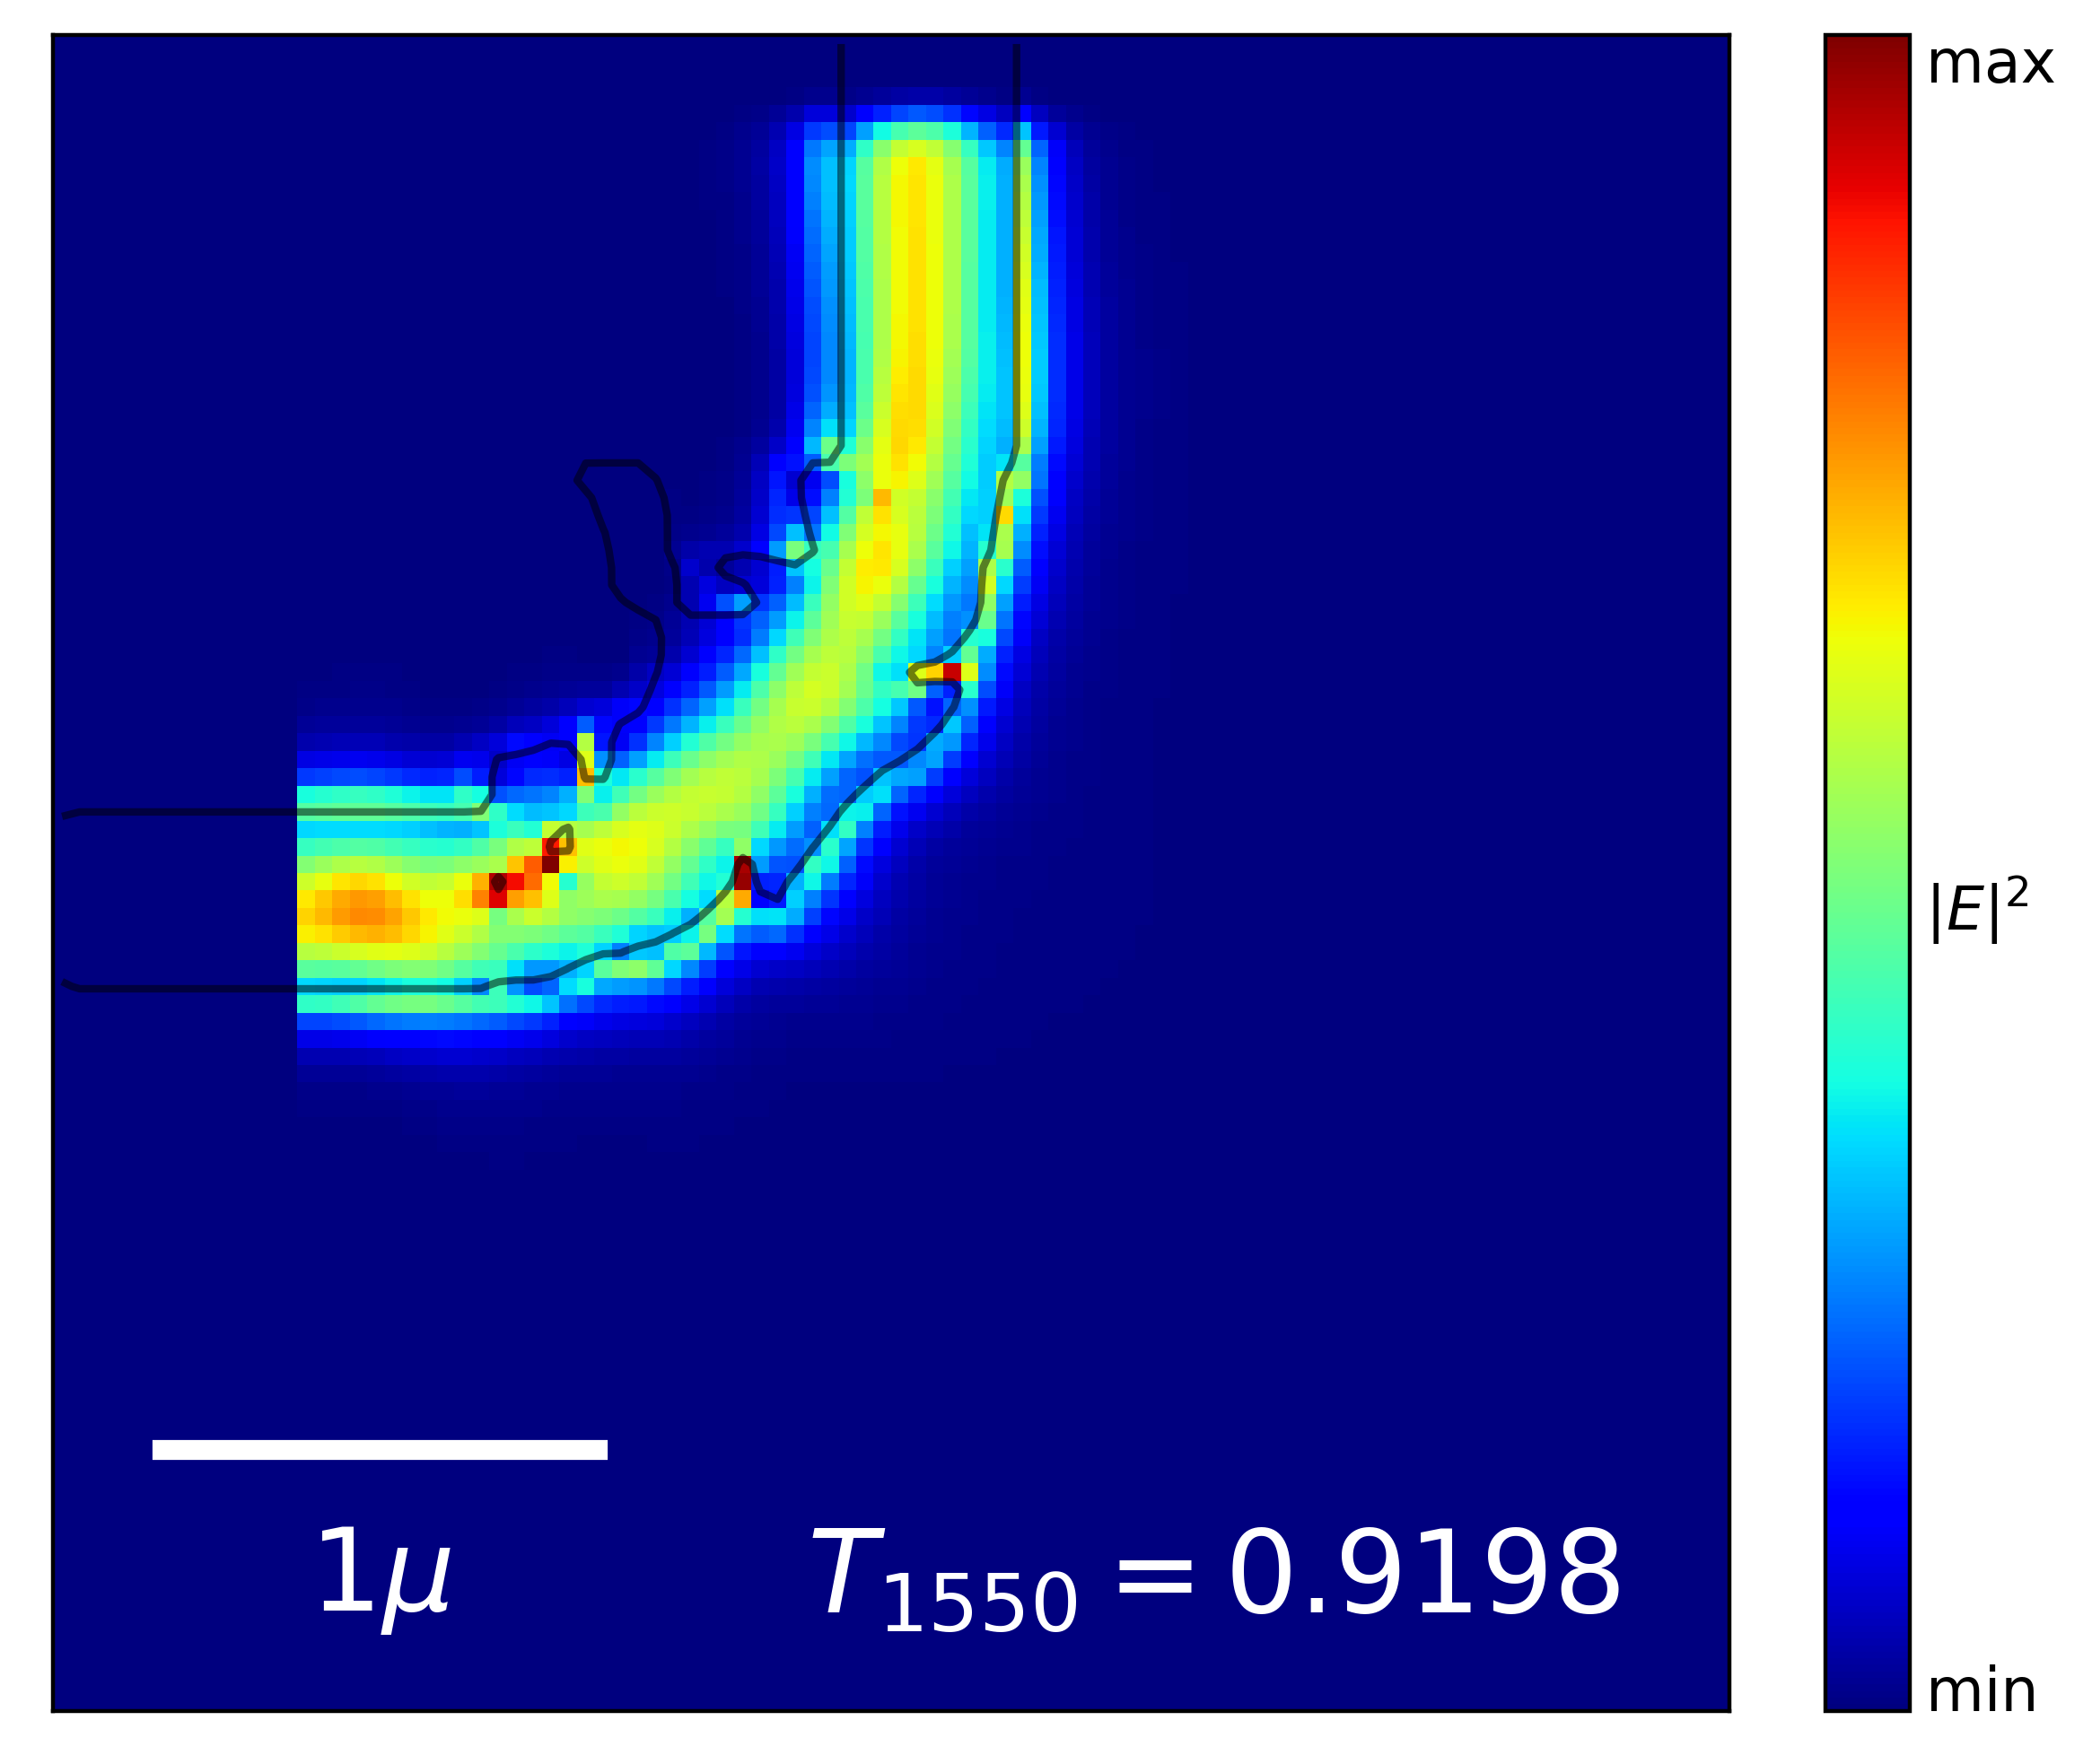
\includegraphics[width=0.35\textwidth]{image/results/bend/best/field_post.png}
  }

  \caption{Posprocesamiento del diseño del \emph{bend} mejor optimizado.}
  \label{fig:bestbend}

\end{figure}

\begin{figure}[ht]
  \centering
  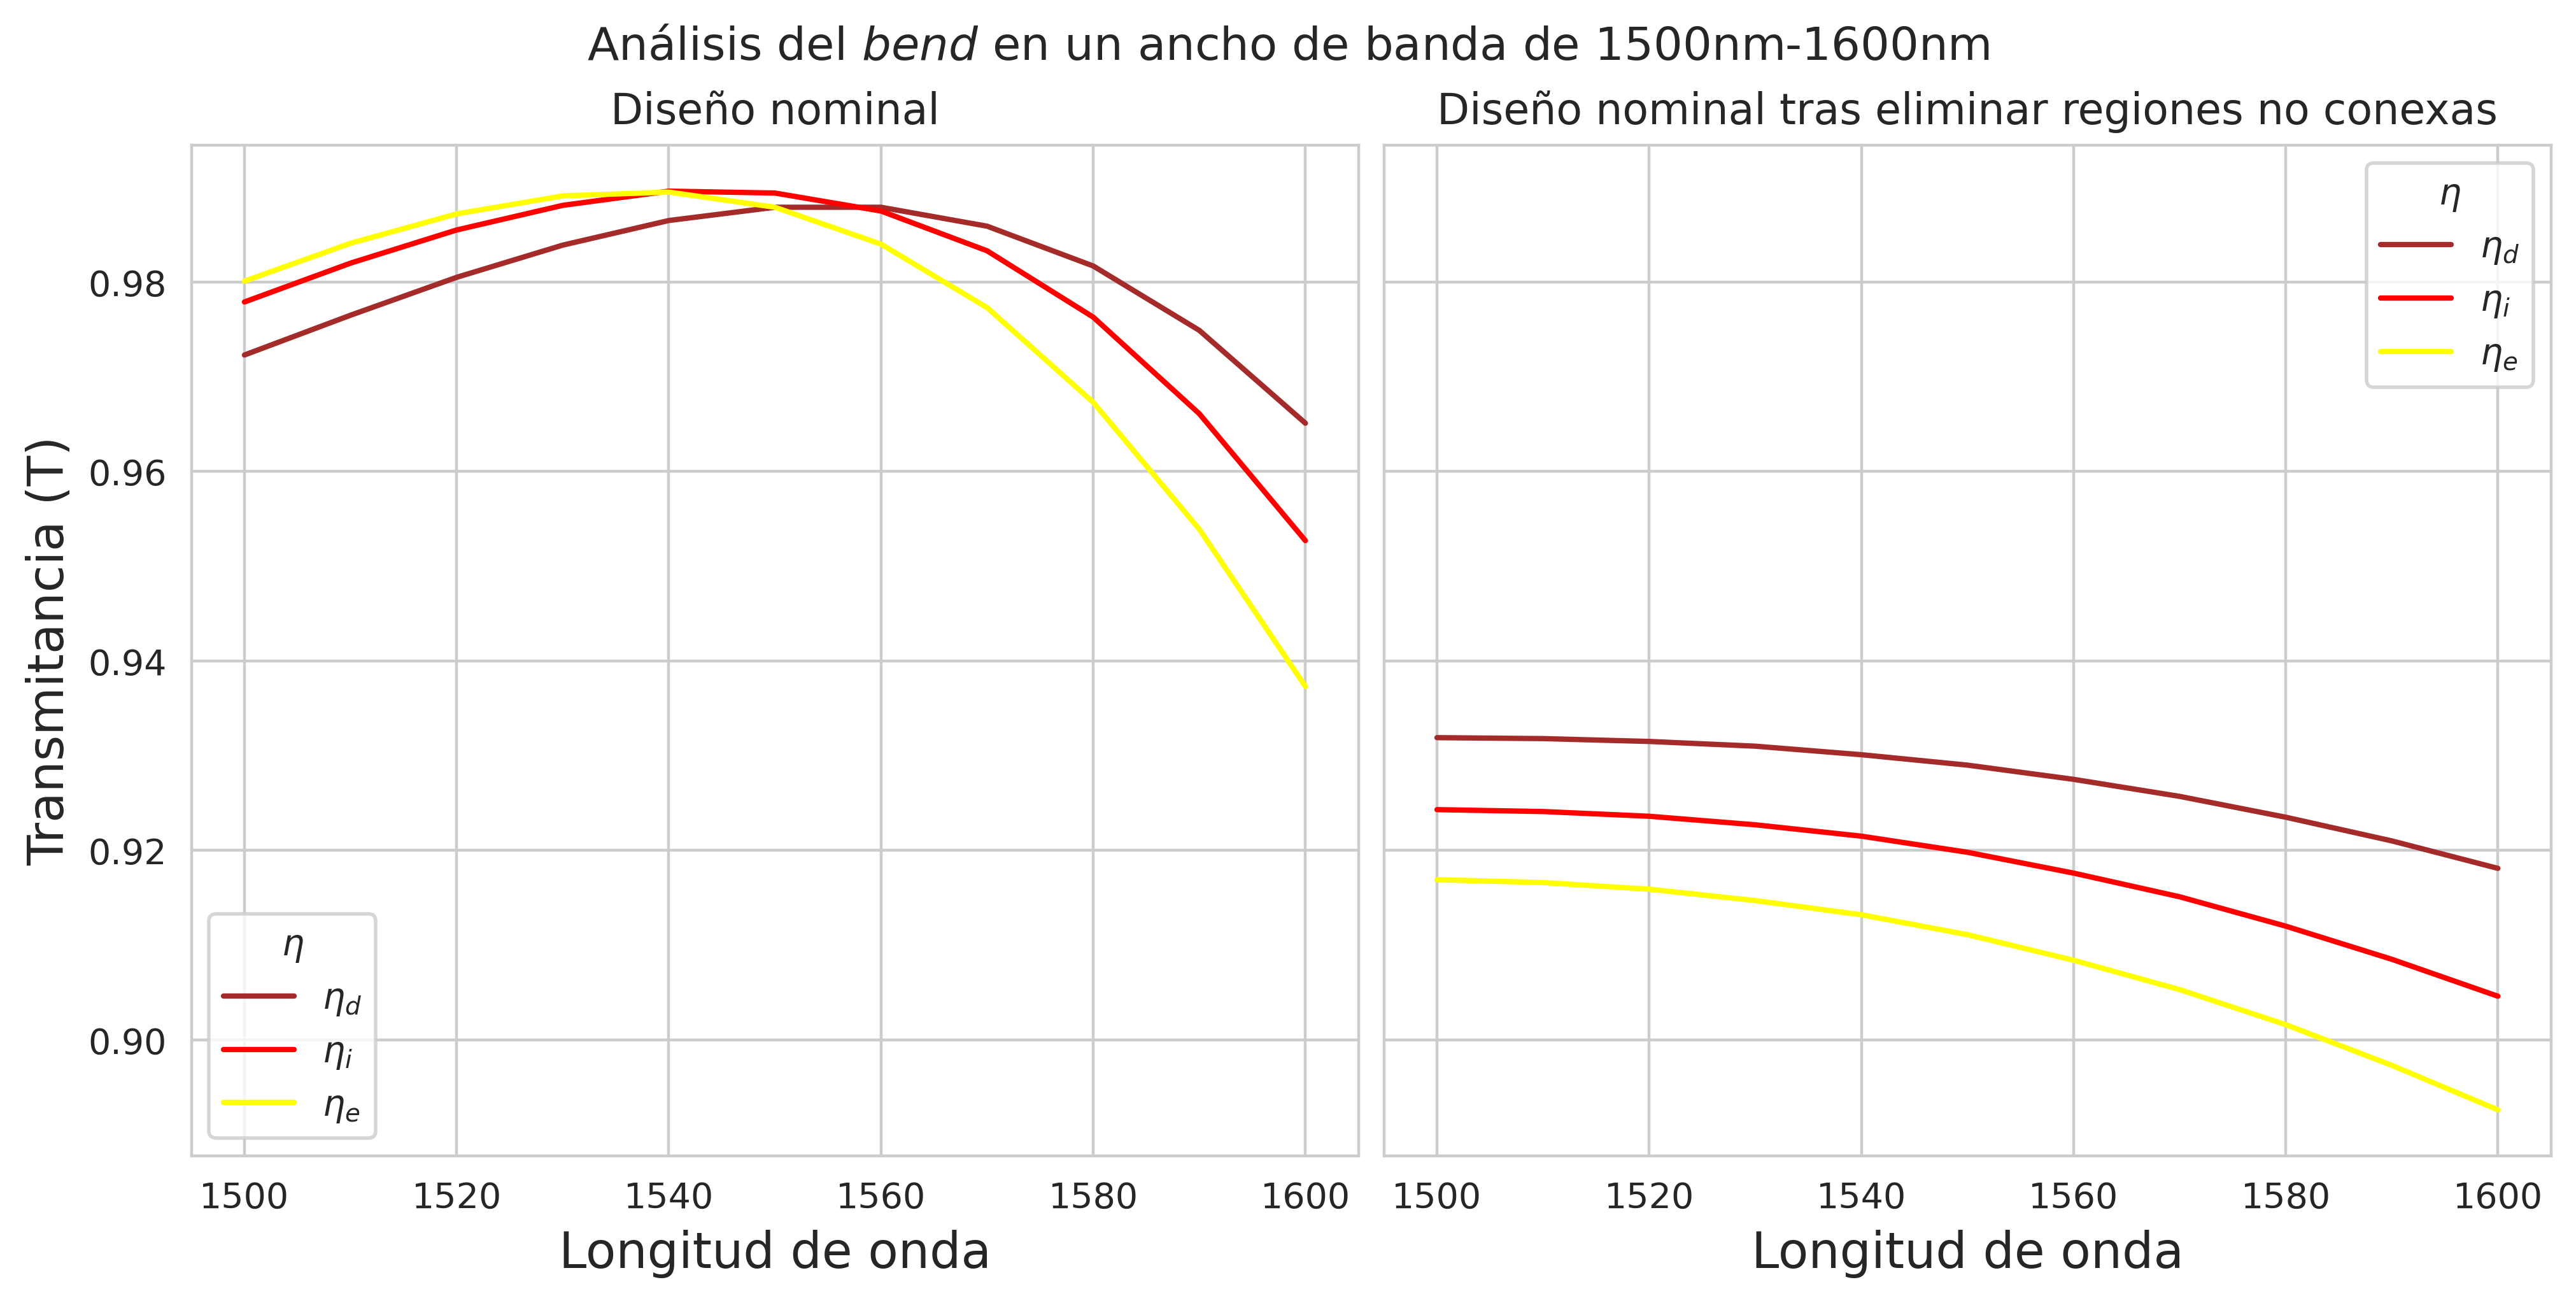
\includegraphics[width=\textwidth]{image/results/bend/best/broadband-bend.png}
  \caption{Análisis del \emph{bend} mejor optimizado en un rango de longitudes de onda ($1500 nm-1600 nm$)}
  \label{fig:broadband-bend}
\end{figure}

\section{Resultados de Optimización del WDM}\label{sec:results-wdm}

En la \autoref{fig:wdm-cont}, \autoref{fig:wdm-disc} y \autoref{fig:wdm-fab} se observa 
el desempeño de los cinco algoritmos seleccionados en la etapa de optimización continua, discreta y
de fabricación del WDM, respectivamente.
Los resultados en más detalle por algoritmo se pueden encontrar en la
\autoref{tab:opt-LBFGSB-wdm} (L-BFGS-B),
\autoref{tab:opt-CMA-wdm} (G-CMA-ES),
\autoref{tab:opt-MMA-wdm} (MMA),
\autoref{tab:opt-PSO-wdm} (G-PSO) y
\autoref{tab:opt-GA-wdm} (G-GA).

\begin{landscape}
\begin{figure}[ht]
  \centering
  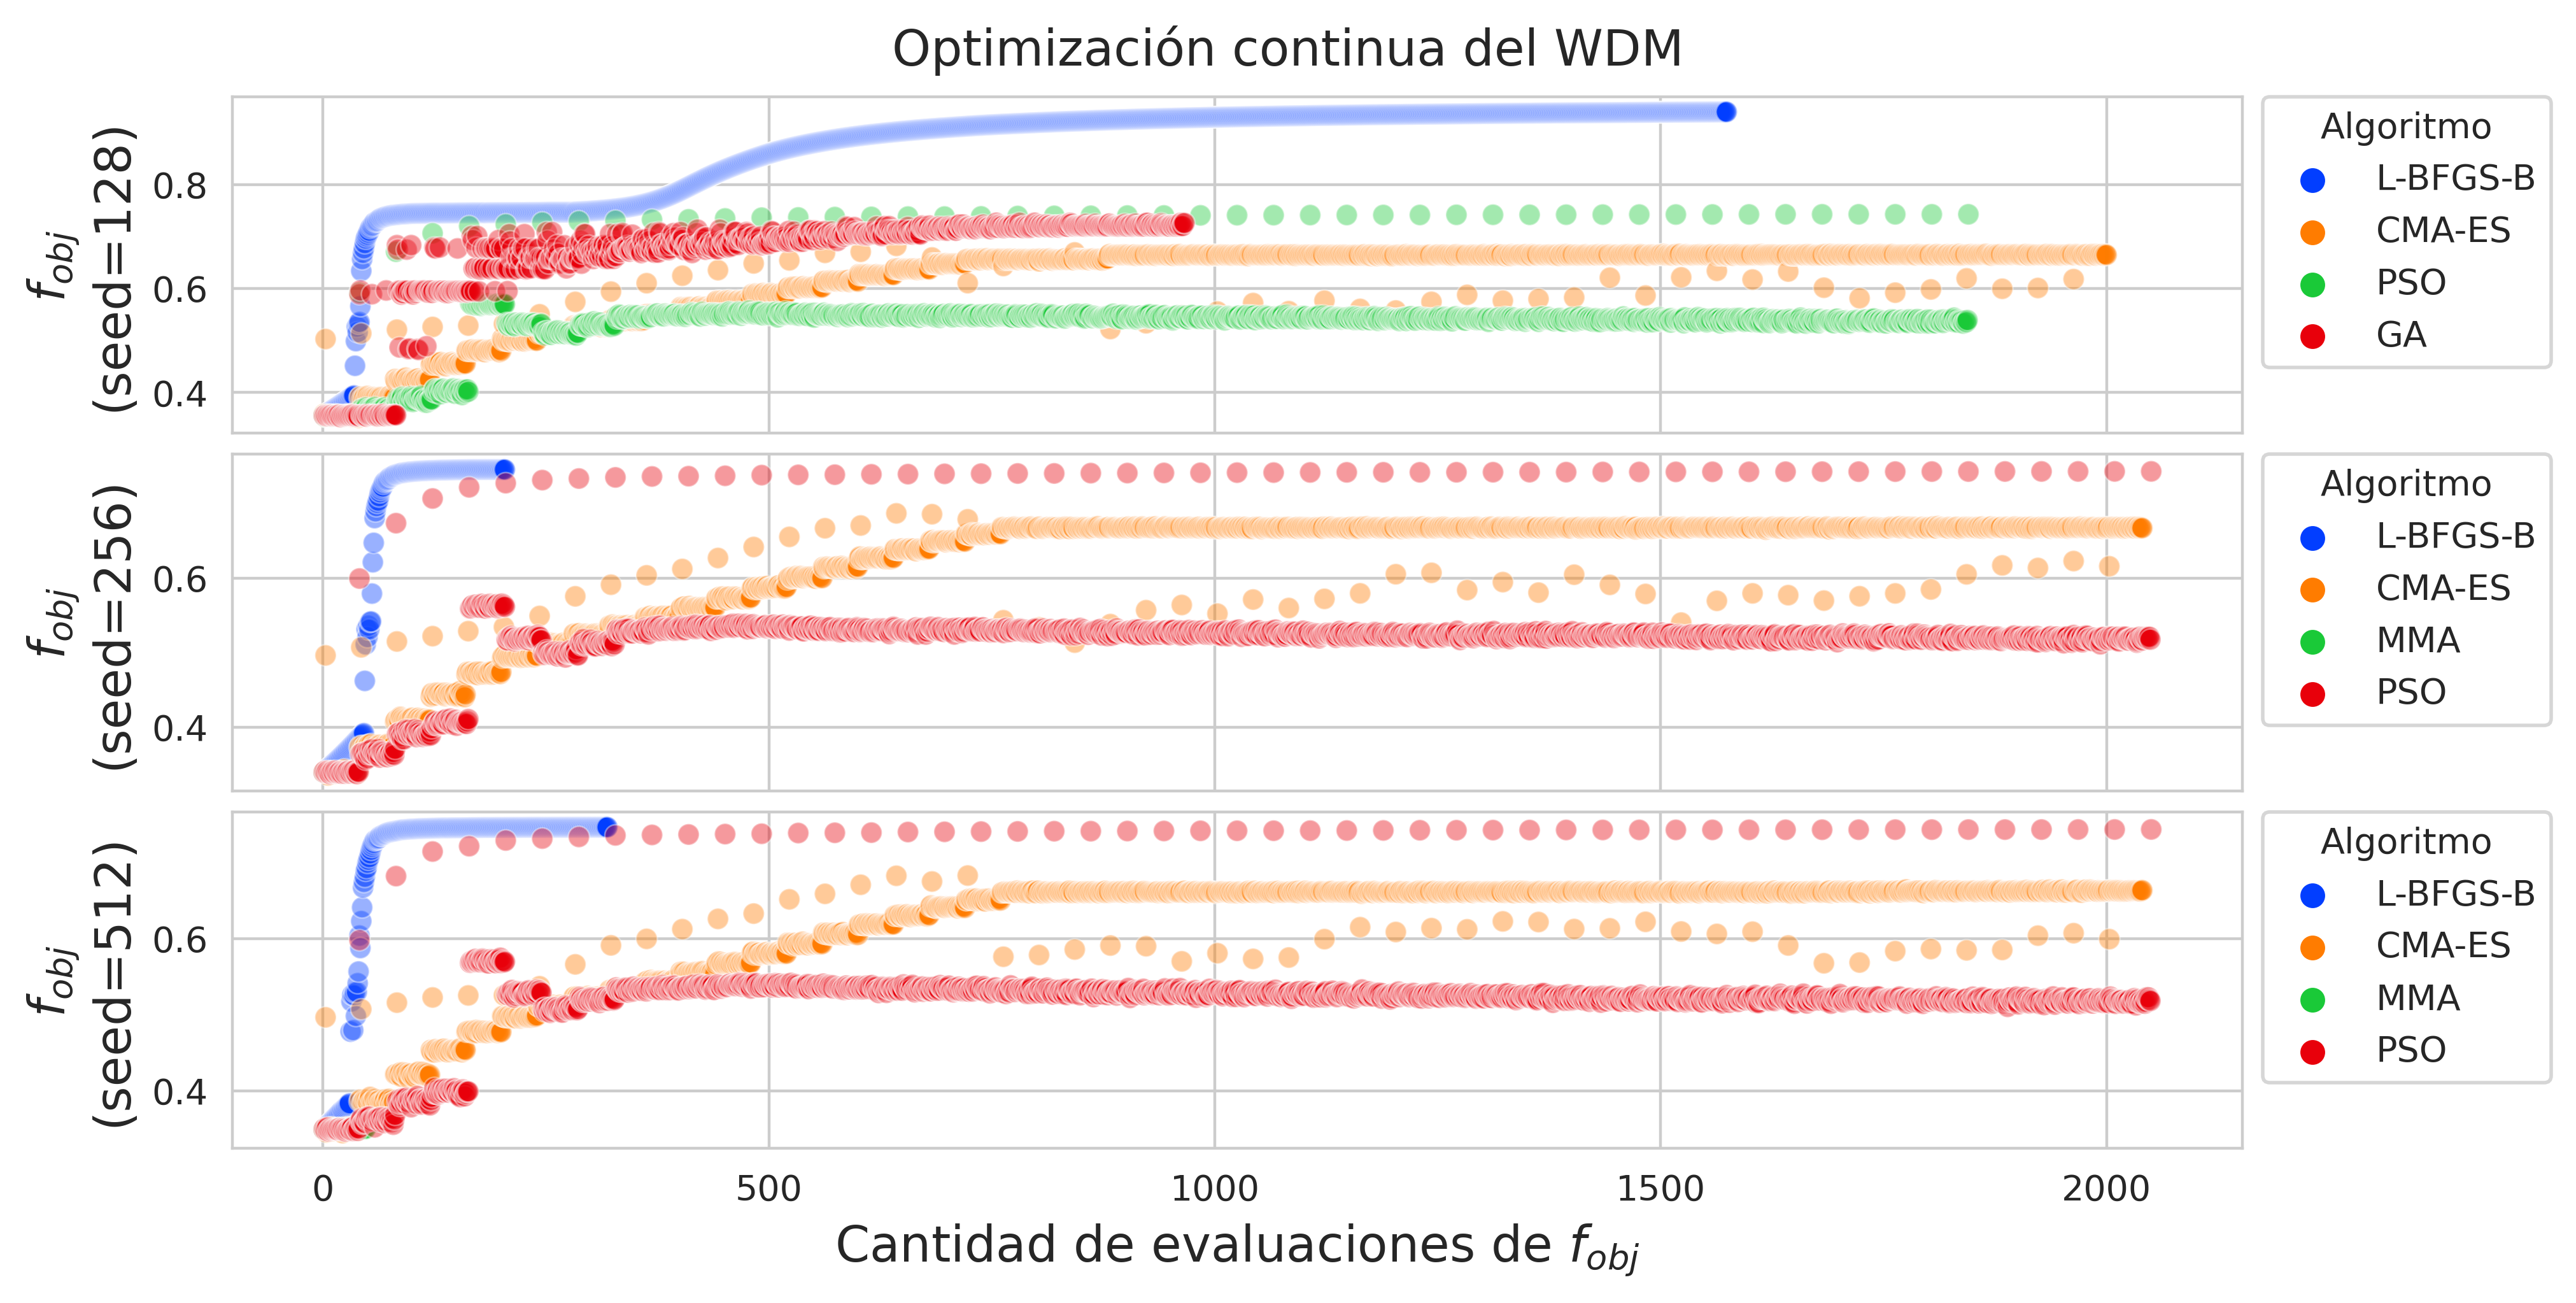
\includegraphics[scale=1.0]{image/results/wdm/wdm-opt-cont.png}
  \caption{Gráfico de valores de $f_{obj}$ obtenidos por los algoritmos en la optimización continua del WDM}
  \label{fig:wdm-cont}
\end{figure}
\end{landscape}

\begin{landscape}
\begin{figure}[ht]
  \centering
  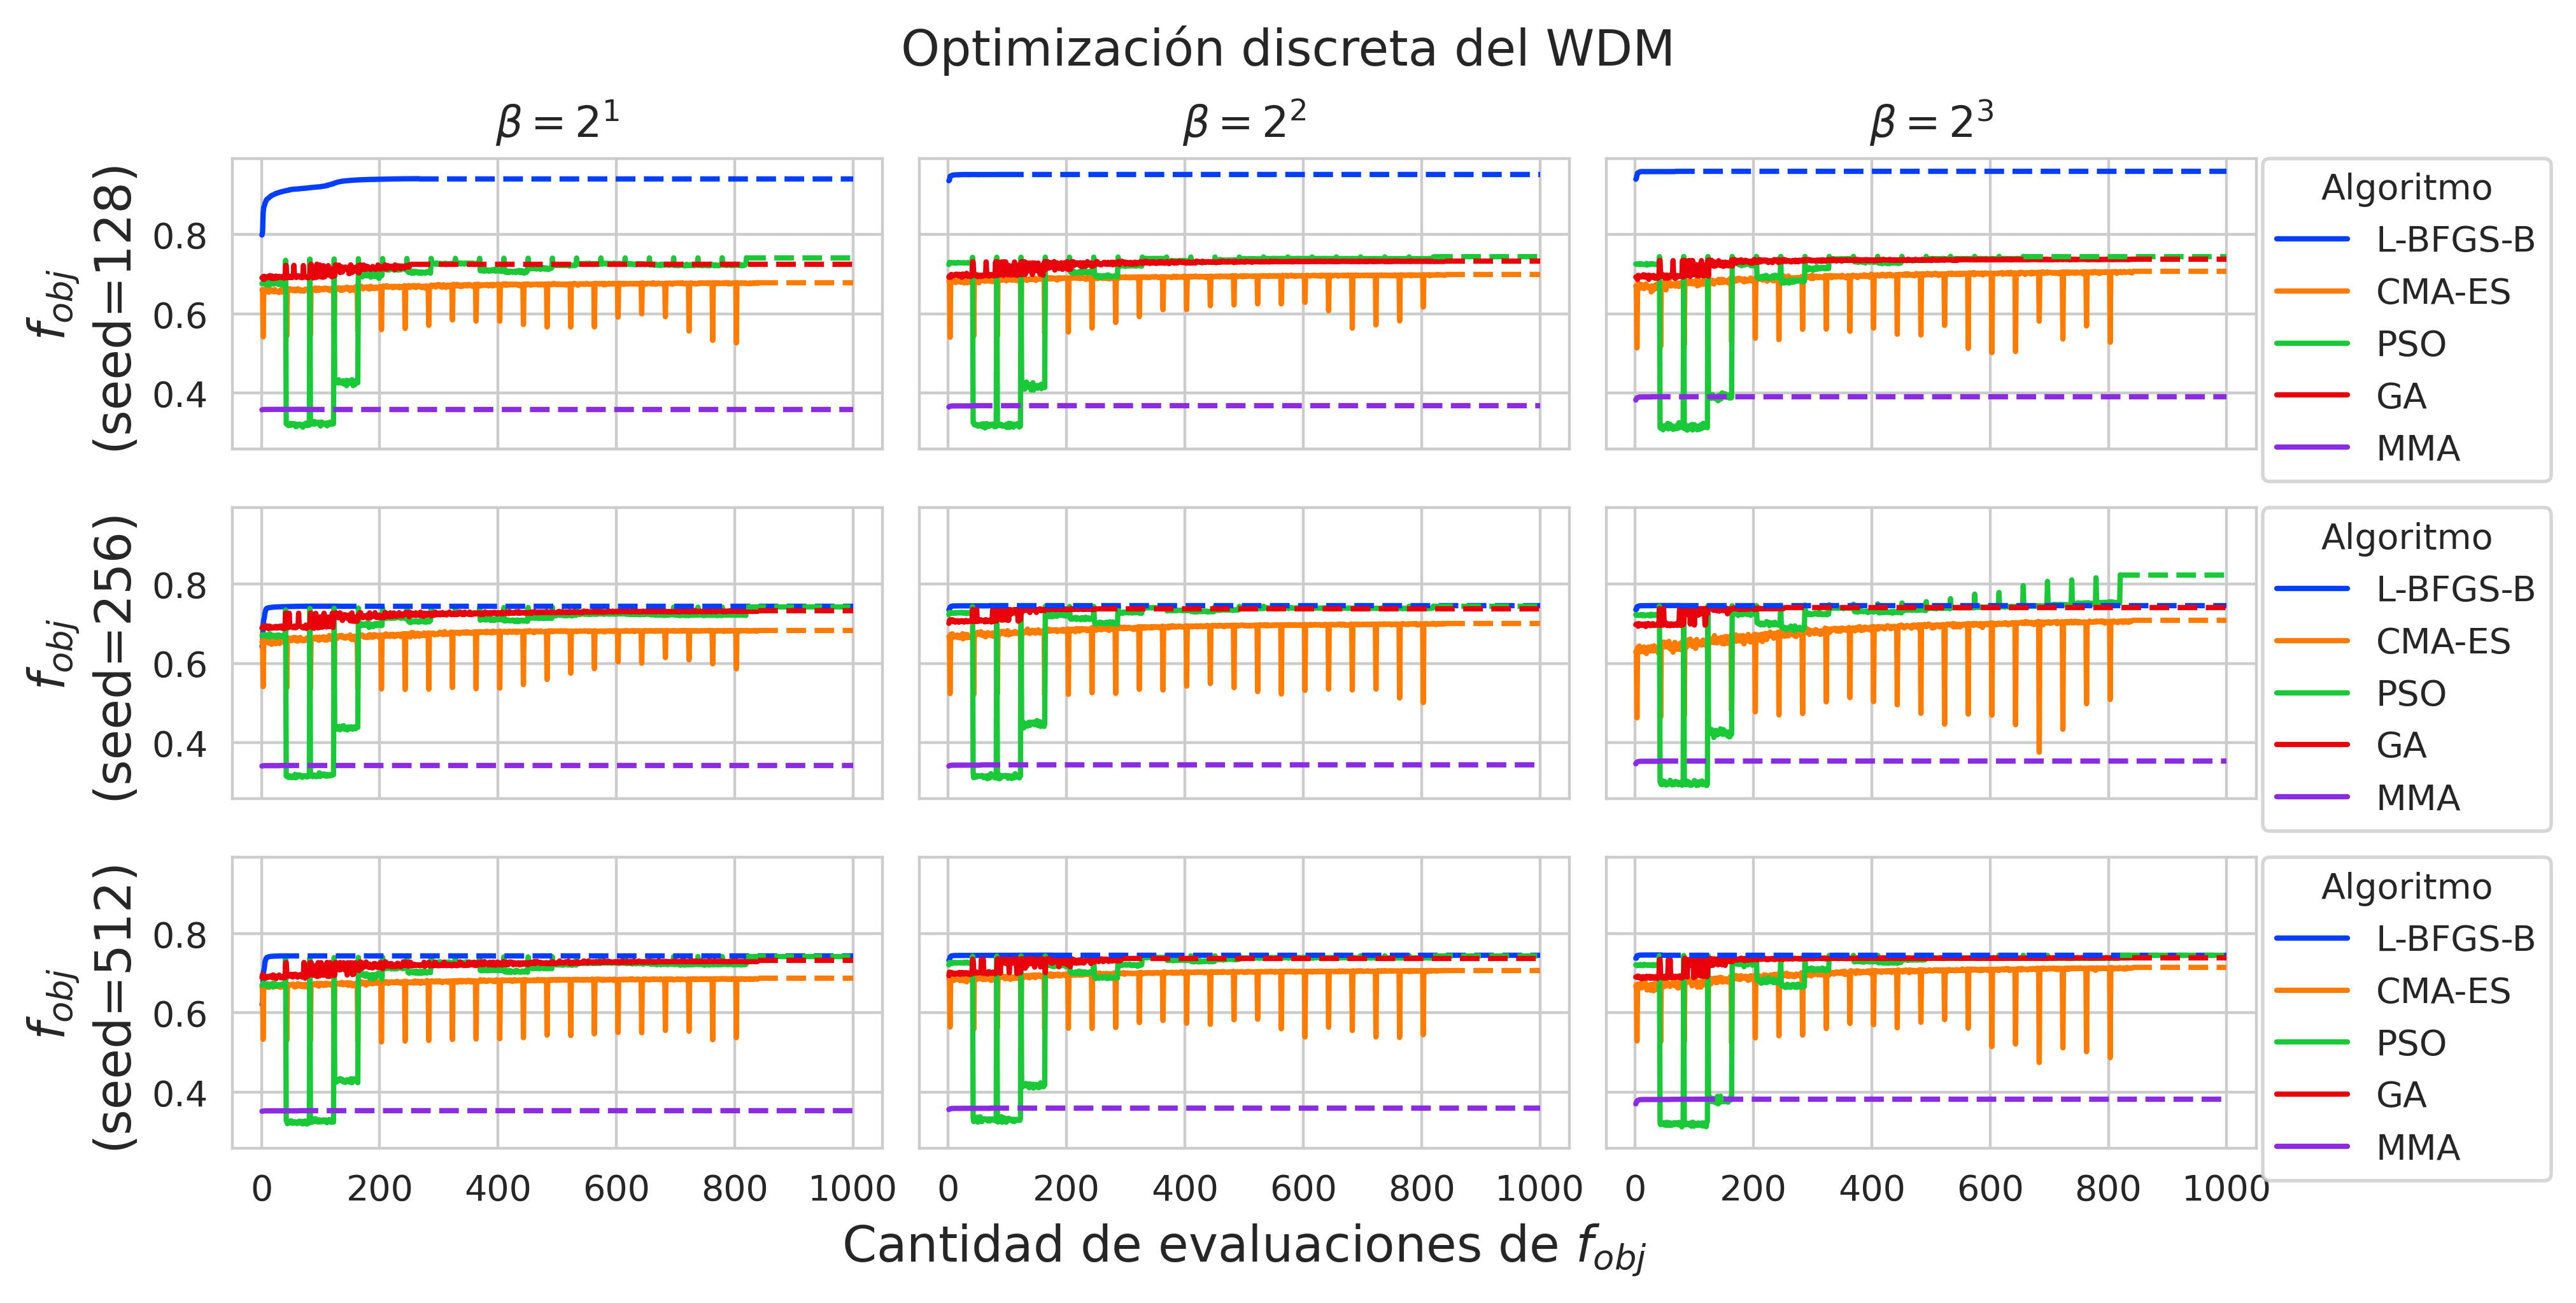
\includegraphics[scale=1.0]{image/results/wdm/wdm-opt-disc.png}
  \caption{Gráfico de valores de $f_{obj}$ obtenidos por los algoritmos en la optimización discreta del WDM}
  \label{fig:wdm-disc}
\end{figure}
\end{landscape}

\begin{landscape}
\begin{figure}[ht]
  \centering
  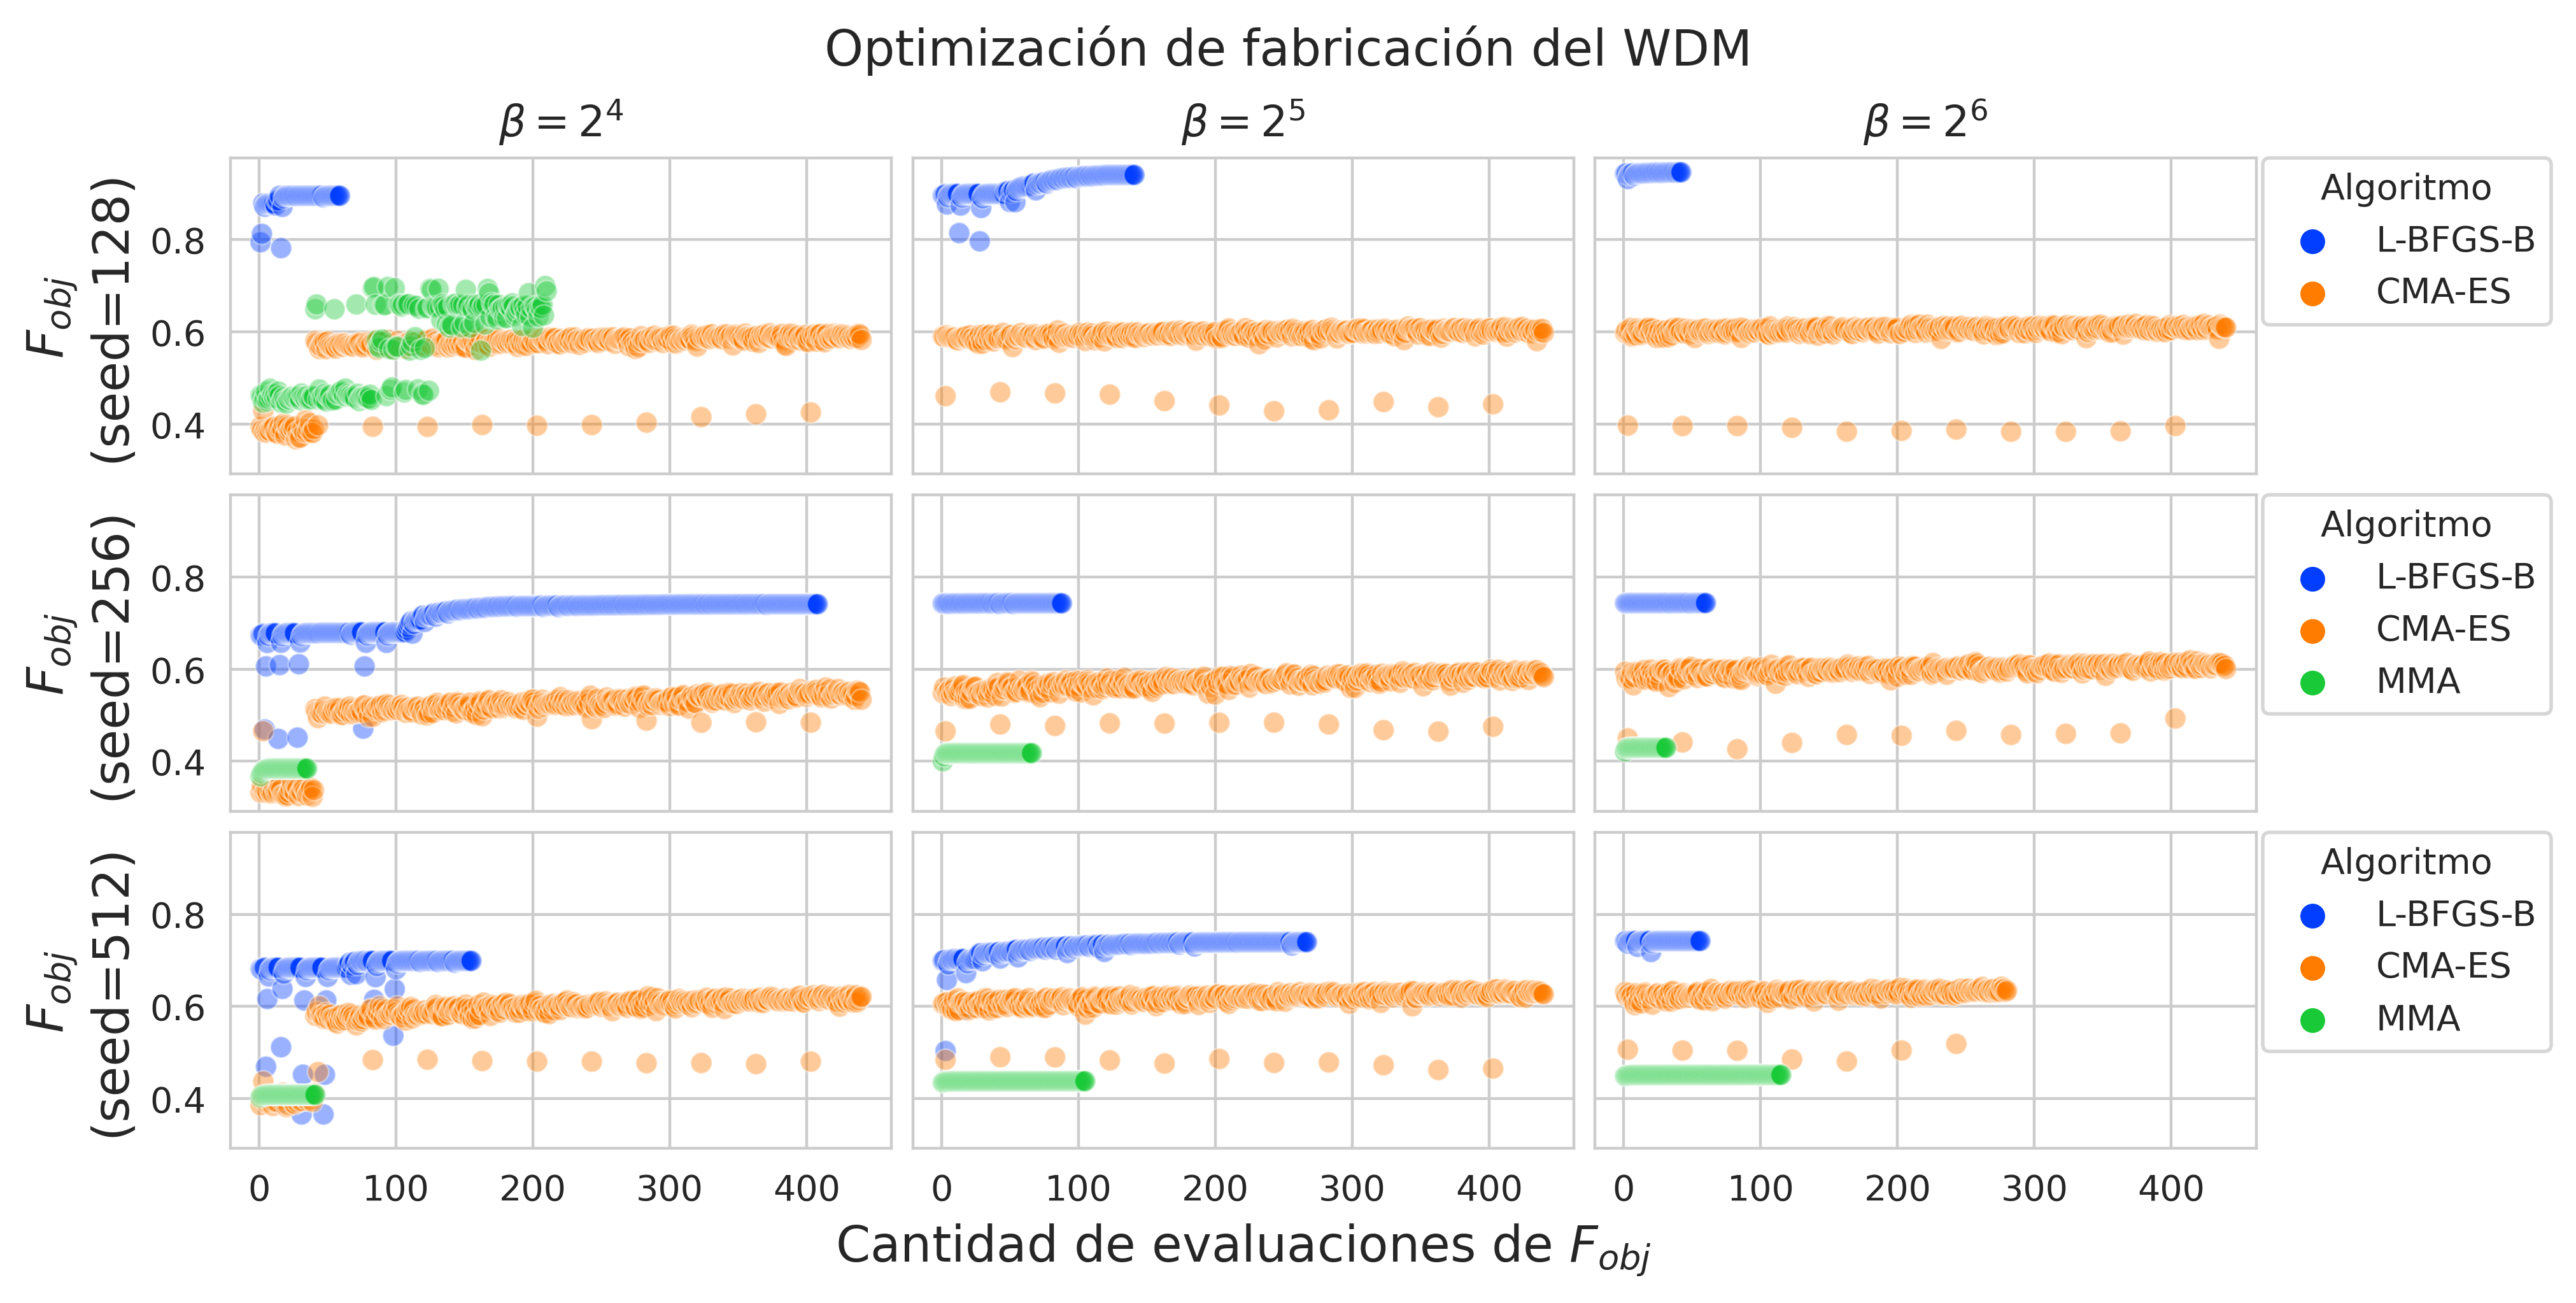
\includegraphics[scale=1.0]{image/results/wdm/wdm-opt-fab.png}
  \caption{Gráfico de valores de $F_{obj}$ obtenidos por los algoritmos en la optimización de fabricación del WDM}
  \label{fig:wdm-fab}
\end{figure}
\end{landscape}

\section{Diseño del WDM Mejor Optimizado}\label{sec:best-wdm}

De la sección anterior tenemos que el WDM mejor optimizado se consiguió
utilizando el algoritmo L-BFGS-B con un \emph{seed} (valor de semilla) de 128.

Al aplicar la \autoref{eq:grayscale} obtenemos que el porcentage de región gris en el diseño
es de 1.233 \%, un valor menor a 2 \%, por lo cual podemos considerar que el diseño ha sido
correctamente binarizado. Por otro lado, si eliminamos las regiones no conectadas con la guía de entrada
tenemos un diseño con un porcentaje de gris de 0.469 \%.
Estos diseños lo podemos observar en la \autoref{fig:bestwdm}.
Adicionalmente, en la \autoref{fig:broadband-wdm} se muestra el comportamiento del diseño
en un rango de longitudes de onda de $1500nm$ a $1600 nm$.

\begin{figure}[ht]
  \centering

  % 1° row
  \subfigure[Diseño nominal.]
  {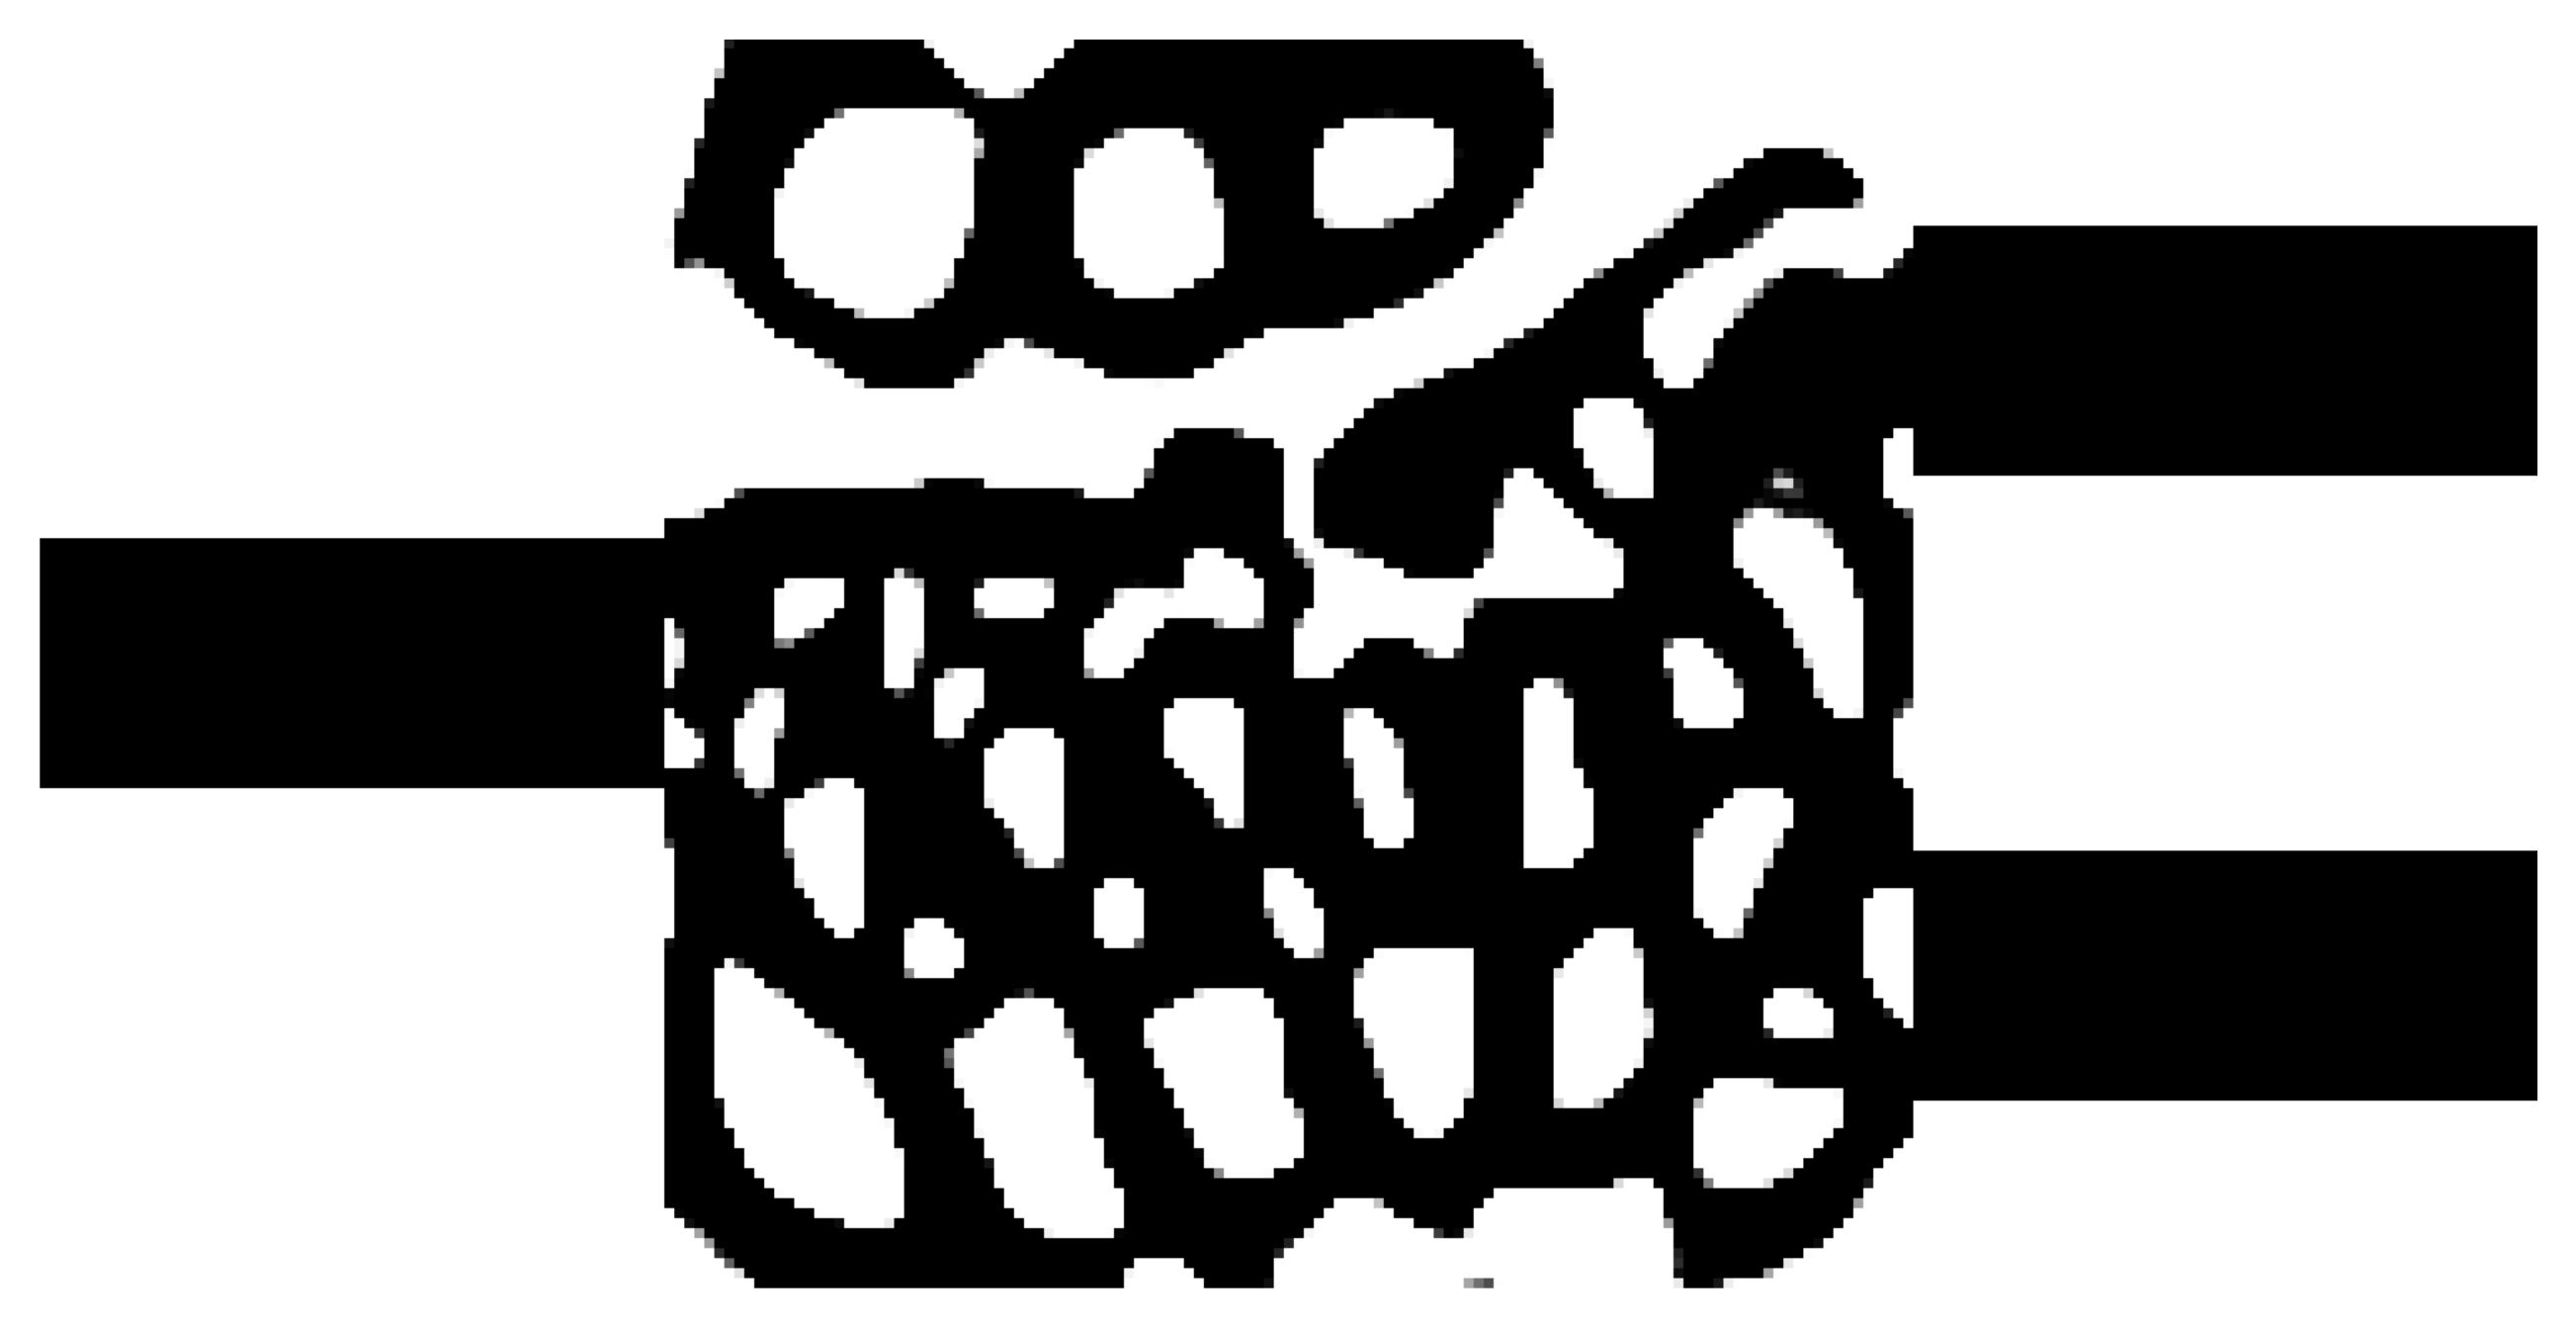
\includegraphics[width=0.45\textwidth]{image/results/wdm/best/eps.png}}
  \hfill
  \subfigure[Diseño nominal tras eliminar regiones no conexas.]{
    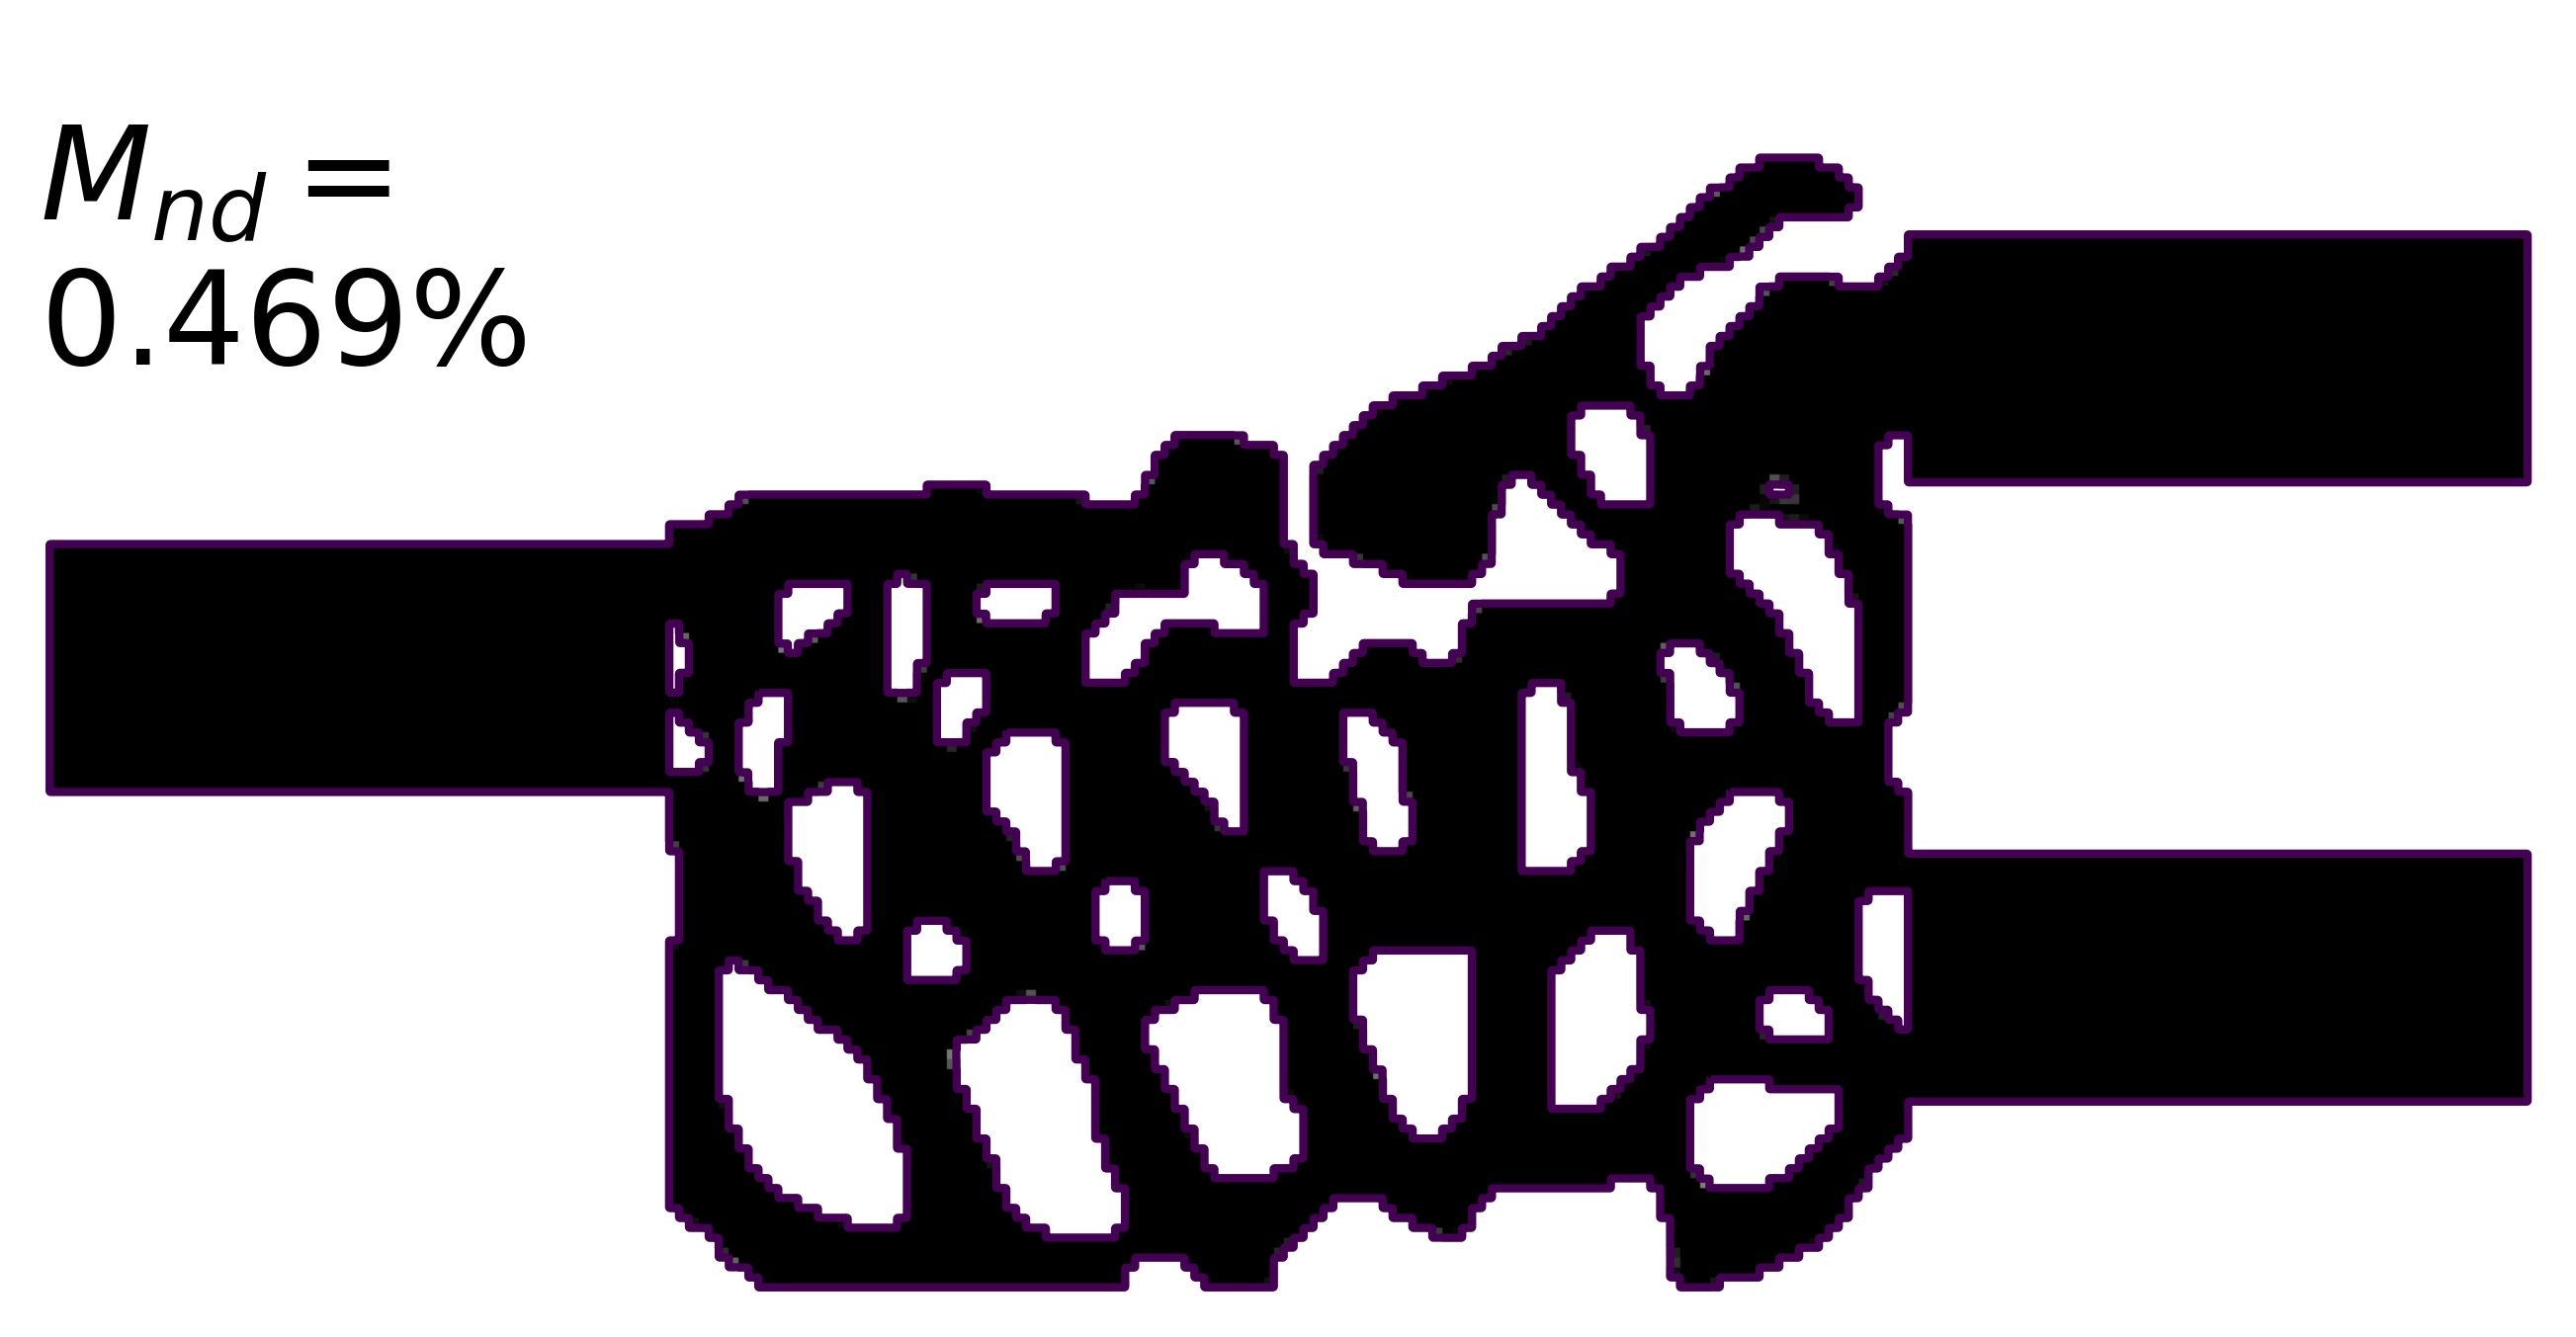
\includegraphics[width=0.45\textwidth]{image/results/wdm/best/eps_post.png}
  }

  % 2° row
  \subfigure[Campo $|\boldsymbol{E}|^2$ del diseño nominal.]
  {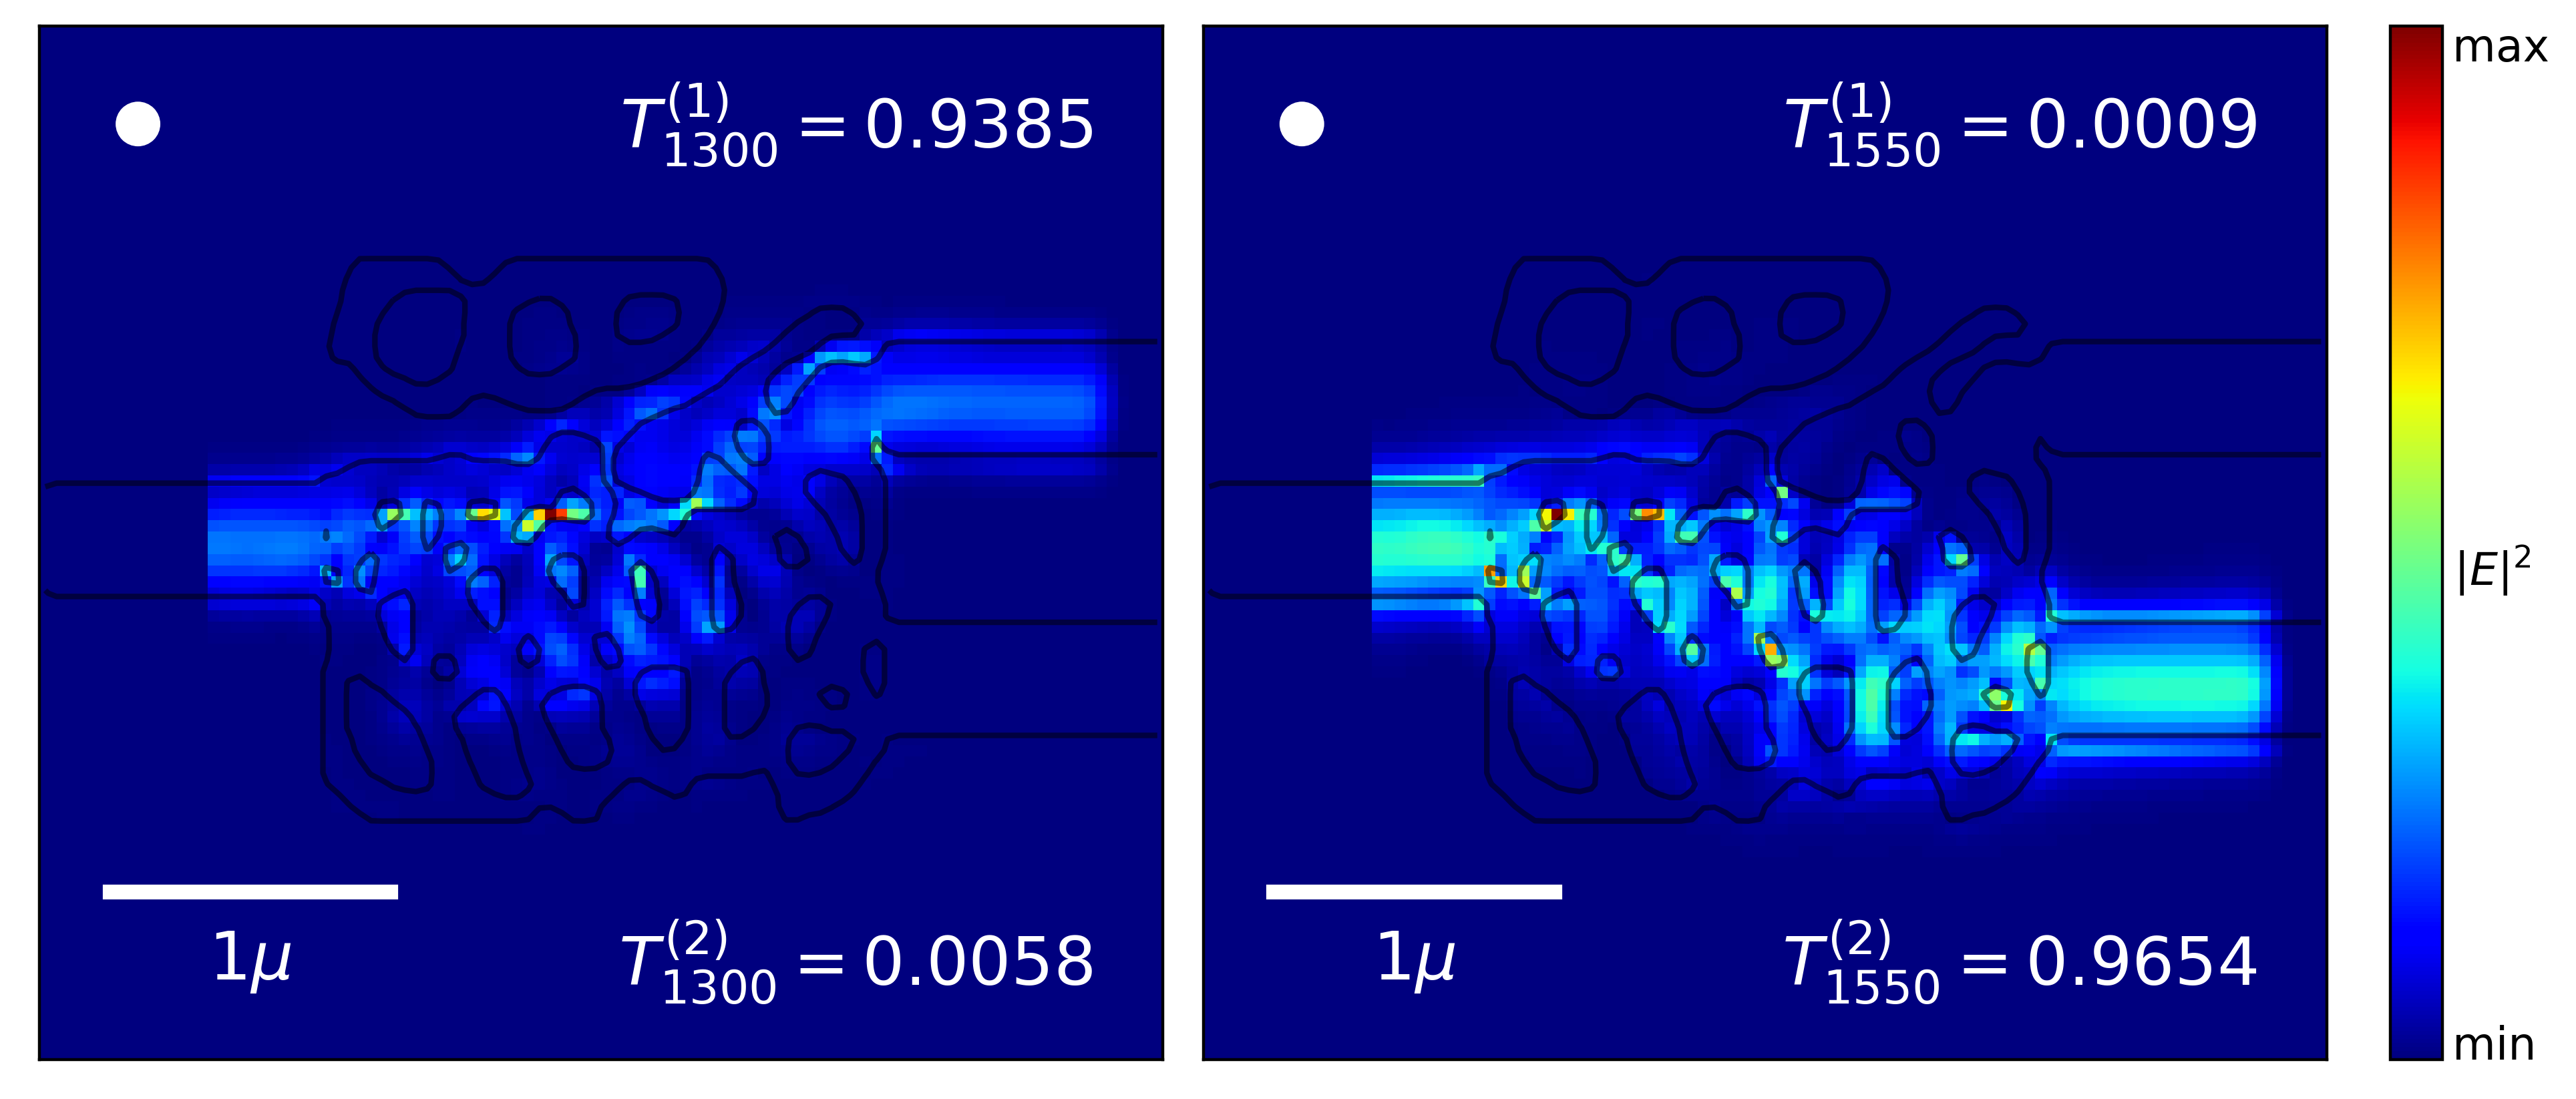
\includegraphics[width=0.45\textwidth]{image/results/wdm/best/field.png}}
  \hfill
  \subfigure[Campo $|\boldsymbol{E}|^2$ del diseño nominal tras eliminar regiones no conexas.]{
    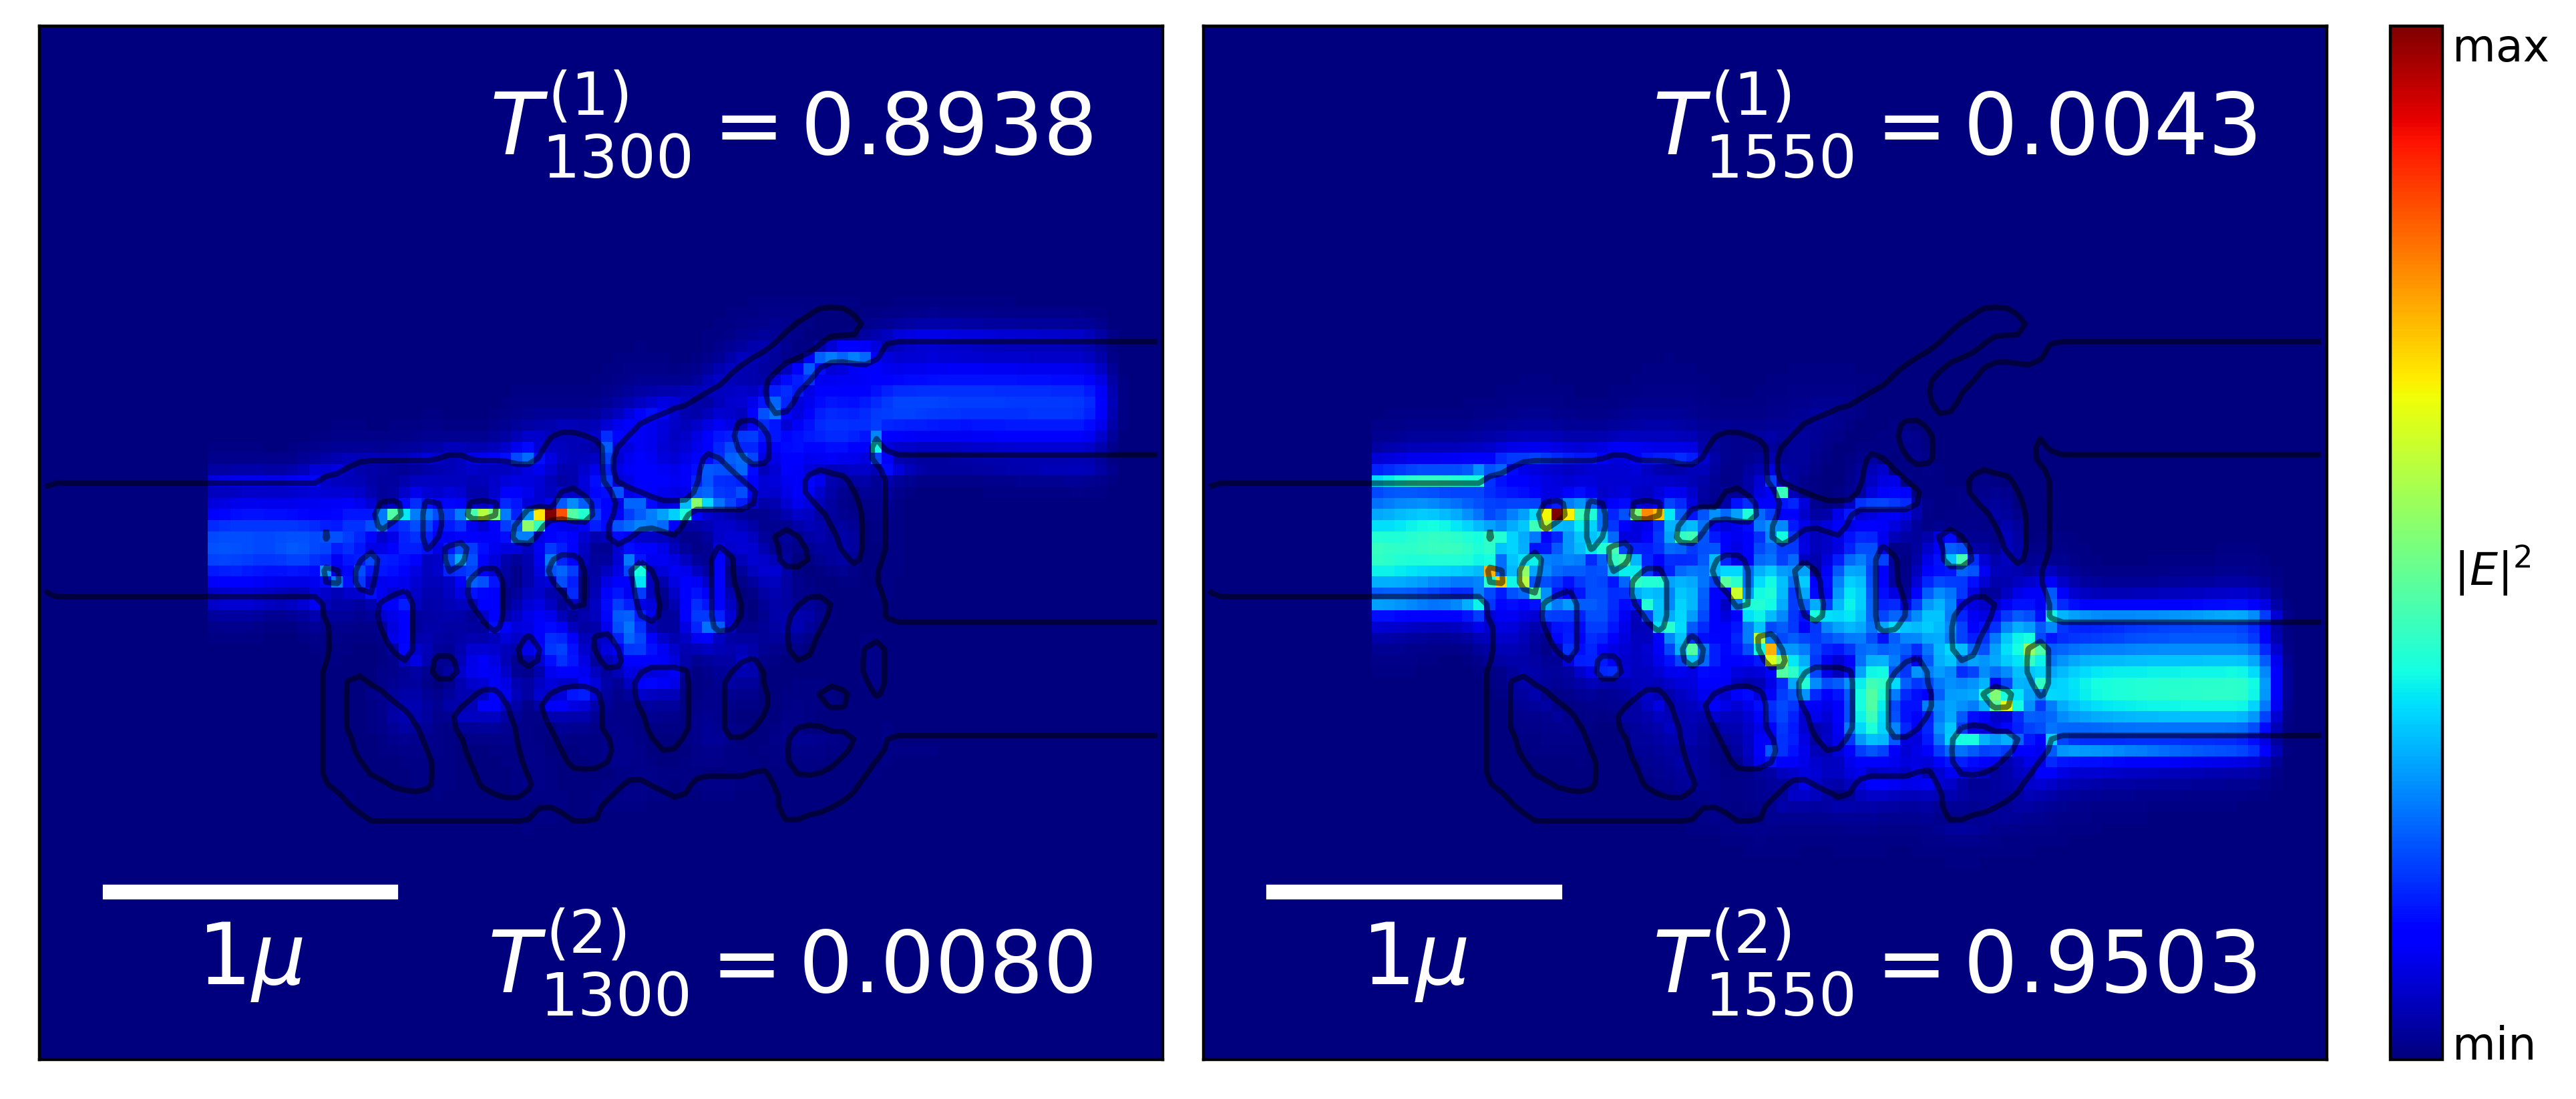
\includegraphics[width=0.45\textwidth]{image/results/wdm/best/field_post.png}
  }

  \caption{Posprocesamiento del diseño del WDM mejor optimizado.}
  \label{fig:bestwdm}

\end{figure}

\begin{figure}[ht]
  \centering
  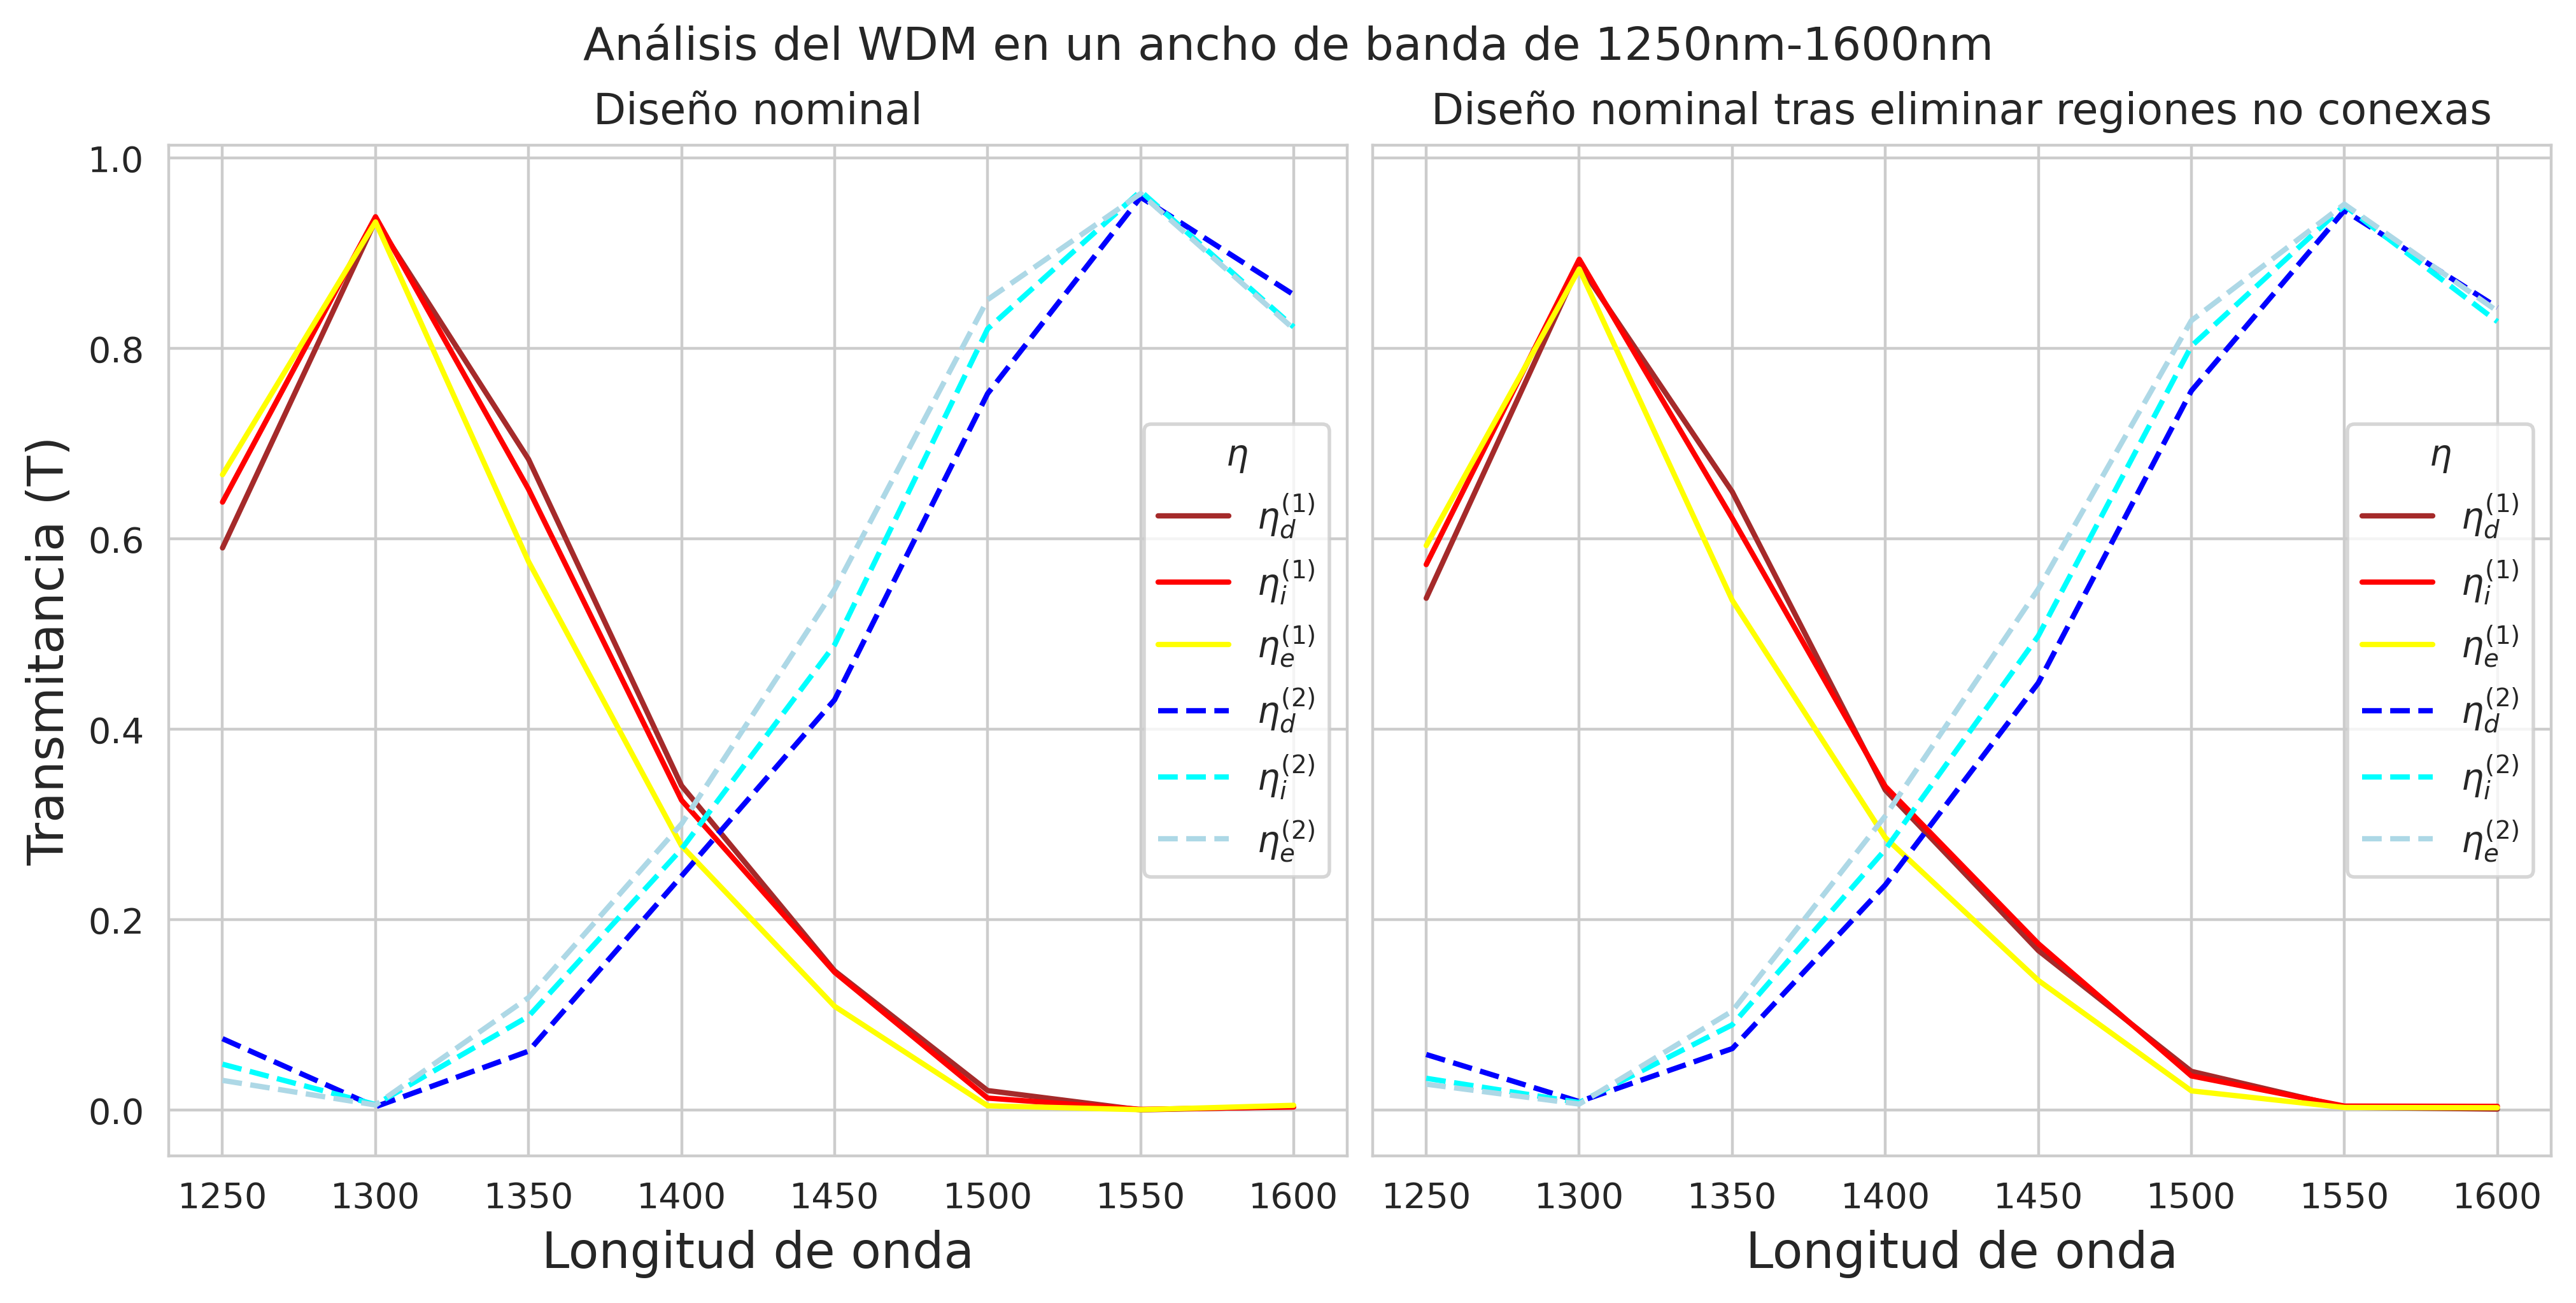
\includegraphics[width=\textwidth]{image/results/wdm/best/broadband-wdm.png}
  \caption{Análisis del WDM mejor optimizado en un rango de longitudes de onda ($1300 nm-1550 nm$)}
  \label{fig:broadband-wdm}
\end{figure}



\section{Discusión de Resultados del \emph{Bend}}

Primero, para poder entender nuestros resultados buscamos una referencia del estado del arte
en la optimización de un \emph{bend}.
Sin embargo, en el mejor de nuestro conocimiento no hay publicaciones recientes que muestren
resultados explícitos en la optimización de un \emph{bend} de un área de diseño de $2 \mu m \times 2 \mu m$.
Pero, utilizando SPINS-B tenemos que el diseño intuitivo posee una transmitancia de $0.8399$ a $1550 nm$.


De la \autoref{sec:results-bend} tenemos que MMA es el único algoritmo que no logra obtener un diseño
mejor que el intuitivo. 
De hecho, todos los demás algoritmos logran una transmitancia de al menos 90 \%.
Particularmente, L-BFGS-B obtiene los mejores resultados y logra una rápida convergencia a un
elevado valor del $FOM$.
Es cierto que G-PSO y G-GA logran una convergencia más rápida. Sin embargo, los 
resultados de estos algoritmos siguen siendo relativamente inferiores a los de L-BFGS-B.

Por otro lado, es interesante destacar que cada algoritmo encuentró geometrías distintas como se
señala a continuación:

\begin{itemize}
  \item L-BFGS-B obtuvo geometrías bien definidas sin gran presencia de regiones puntiagudas.

  \item G-CMA-ES obtuvo geometrías con presencia de pequeñas zonas grises y zonas puntiagudas.

  \item MMA obtuvo diseños que no lograron conectar las guías de onda.

  \item G-PSO logró encontrar diseños compactos y evitó obtener islas pequeñas.

  \item G-GA por su lado tuvo un comportamiento similar a G-PSO.

\end{itemize}

Curiosamente, sin contar al MMA, los algoritmos producieron pequeñas islas.
En la \autoref{sec:best-bend} se utilizó el diseño mejor optimizado para experimentar
quitando estos elementos. Sorprendentemte, estos resultados siguieron teniendo una transmitancia
mayor a 90 \%.
Incluso si trabajamos en longitudes de onda en el rango de $1500nm-1600nm$
los resultados se mantienen similares aún cuando pueda ocurrir errores de erosión o dilatación.
De este modo, se comprueba que el diseño obtenido es eficiente y robusto no solo a errores
de fabricación, sino que también es flexible en la longitud de onda con la que puede trabajar.

\section{Discusión de Resultados del WDM}

Para poder entender nuestros resultados buscamos una referencia del estado del arte en la optimización
de un WDM. Así, tenemos:

\begin{itemize}
  \item \cite{Christiansen2021} optimizaron un WDM con una región
  de diseño de $2 \mu m \times 2 \mu m$ trabajando a $1300 nm$ y $1550 nm$ logrando obtener un diseño
  con $T_{1300}^{(1)} = 0.86$ y $T_{1550}^{(2)} = 0.85$.

  \item \cite{Piggott2015} optimizaron un WDM con una región de diseño de $2.8 \mu m \times 2.8 \mu m$
    trabajando a $1300 nm$ y $1550 nm$. En su trabajo muestran los resultados en gráficas por lo cual
    es dificil encontrar los valores de transmitancia exactos reportados. Sin embargo, en
    \cite{Sigmund2016} se detalla que el diseño obtenido posee 
    $T_{1310}^{(1)} = 0.8377$ y $T_{1550}^{(2)} = 0.8076$.
\end{itemize}

El diseño del WDM mejor optimizado en este trabajo posee $T_{1300}^{(1)} = 0.9385$ y 
$T_{1550}^{(2)} = 0.9503$ y tras eliminar las regiones no conexas obtiene
$T_{1300}^{(1)} = 0.8938$ y $T_{1550}^{(2)} = 0.9503$. Además, al realizar el análisis
en un rango de longitudes de onda de $1250nm-1600nm$ obtenemos un comportamiento similar
al logrado en \cite{Piggott2015}.
De este modo, aparentemente hemos obtenido un diseño que supera el estado del arte.
Sin embargo, es necesario fabricar estos diseños para corroborar los resultados de las simulaciones.

Por otro lado, de la \autoref{sec:results-wdm}, tenemos que al igual que sucedió con el \emph{bend},
MMA no está logrando llegar a diseños que al menos conecten las guías de onda.
Primero, se consideró la posibilidad de haber algún error en el cálculo de la gradiente;
sin embargo, los demás algoritmos si han logrado tener éxito en la optimización tanto del \emph{bend}
como del WDM. Así, este escenario es poco probable.
Además, para la configuración del algoritmo se utilizó como guía un tutorial de MEEP \citep{Oskooi2010},
por lo que un error de configuración también parece sensato de descartarse.
Probablemente, el algoritmo simplemente requería de una cantidad mayor de iteraciones.


Respecto al desempeño de los demás algoritmos, es importante señalar que si bien todos lograron
conectar las guías de onda, estos prefirieron mantener la guía de salida superior disconexa.
El diseño mejor optimizado (L-BFGS-B con valor de semilla de 128) es el único que logra conectar
la guía de entrada con ambas guías de salida.
En general, podemos interpretar este buen resultado como un caso particular.
Parece sensato concluir que la definición de nuestra función objetivo aún carece de un
término que incentive a que ambas guías de salida queden conectadas.


Sobre la convergencia de los algoritmos, de la \autoref{fig:wdm-cont}, \autoref{fig:wdm-disc}
y \autoref{fig:wdm-fab} queda evidente que L-BFGS-B supera a los demás algoritmos en términos
de convergencia y mejores valores alcanzados.
Además, se puede observar que tanto G-PSO como G-GA presentan comportamiento similares y ambos
superan a G-CMA-ES en términos de mejores valores alcanzados.
Particularmente, como se muestra en \autoref{fig:wdm-cont}, CMA-ES parece caracterizarse
por mejorar de manera lenta, mientras que los demás algoritmos (a excepción de MMA) logran tener
mejoras bruscas al inicio de la optimización.


Finalmente, es interesante destacar que las geometrías encontradas por cada algoritmo muestran
características en común con los resultados encontrados en la optimización del \emph{bend}.
Por un lado, L-BFGS-B, G-PSO y G-GA han encontrado geometrías sin gran presencia de regiones puntiagudas.
Por otro lado, G-CMA-ES obtuvo diseños con regiones puntiagudas y regiones disconexas muy pequeñas.
Y, MMA no logró concretar ninguna geometría, el resultado de obtener ciertas regiones definidas parece
ser simplemente el producto de las transformaciones en un diseño aleatorio.


En este capítulo hemos desarrollado la propuesta presentada en el \autoref{chapter:methodology}.
Primero, se realizó una descripción de los resultados de la optimización del \emph{bend} y 
se analizó al mejor diseño obtenido. 
Luego, se practicó la misma estrategia sobre los resultados del WDM.
Finalmente, hemos realizado una discusión crítica sobre estos resultados.
Así, como hemos podidos observar, hemos conseguido diseños eficientes y robustos tanto para un \emph{bend}
como para un WDM siguiendo la estrategia de optimización planteada.
